%*******************************************************************************
%****************************** Second Chapter *********************************
%*******************************************************************************

\chapter{A new Peierls model}
\label{chap:peierls_model}
\graphicspath{{peierls_model/Figs/}}

\epigraph{Calculations are made of the size of a dislocation}{\emph{R.E. Peierls}}


Though there are a number \cite{Nabarro1947,Huntington1955, puls1976, Vitek1992,  Bulatov1997, Lubarda2007, Clegg2006,Gouriet2015} of Peierls models published in the literature over the decades since \citet{Peierls1940} first presented his solution, few have been applicable to situations beyond the initially envisaged problem, which is somewhat narrowly defined for an orthorhombic lattice that obeys linear elasticity. In this chapter a model is presented that allows  the consideration of energies defined by linear elasticity using the full elastic tensor, empirical potentials and generalised stacking fault energies. The model is also kept modular to allow extension to other formulations, e.g. a full quantum mechanical treatment using density functional theory.

This model does not aim to radically deviate from all the previous work on the Peierls model, there is no need to as much progress has been made over the years. Instead this new model aims to bring together as much of that previous work as possible to try and provide new insight into the behaviour of dislocations. For example, the use of ionic empirical potentials is not new, \cite{Hoagland1976}, and neither is the idea of fitting a misalignment potential and numerical optimisation of the structure rather than closed form solutions \cite{Bulatov1997}, others have considered a more generalised displacement field \cite{Lubarda2007} and the full elastic stiffness tensor has been used since very early in the study of dislocations \cite{Eshelby1949}. There is however scope to further combine these different factors, along with more powerful computers in the modern era, to provide a more generalised model while relaxing the assumptions and simplifying constraints enough to provide insights into unusual dislocation behaviour.

The Python programming language was chosen for a number of reasons. Firstly the Python model is inherently modular, which provides a flexible structure, allowing parts of the model to be altered, extended or replaced quickly and easily. Secondly Python is also widely used for scientific computing, with a comprehensive body of documentation and a large support community. Finally Python has a very large number of extending modules providing advanced capabilities, particularly projects like NumPy and SciPy. NumPy provides a powerful and efficient implementation of arrays and a range of simple functions as well as more advanced linear algebra operations. SciPy is a project built on the basic data structure of the NumPy array and provides advanced algorithms and convenience functions including differential equations, numerical solvers and optimisers, image processing and statistical functions. The code written in this work has been published on-line \cite{code}. 

To calculate the Peierls stress we must find the changes in the dislocation energy as a dislocation moves from one low energy position to the next. The variable $\alpha$ is used to denote the  displacement of the dislocation as a fraction of the Burgers vector, $b$. Since boundary conditions are insufficient to define the atomic configuration, for each value of $\alpha$ the atomic configuration of the dislocation that minimises the energy must be found. Once sufficient samples of $\alpha$ have been made the Peierls stress can be calculated by:
\begin{equation}
\tau_p = \frac{1}{lb^2}   \left. \frac{\partial U}{\partial \alpha} \right|_{max} .
\end{equation}
where $l$ is the length of dislocation line for which the energy, $U$, is calculated for and $b$ is the Burgers vector.

For a given value of $\alpha$ the lowest energy configuration is found via three steps: first the definition, creation and representation of an atomic configuration, second the evaluation of the overall energy, and third the iterative improvement of the configuration to find the minimum energy. Taken together the first two steps can be thought of as a function that takes the value of $\alpha$ along with some input parameters as arguments and returns the total energy:

\begin{equation}
U_{\text{total}} = f(\alpha, p_1, p_2,...,p_n )
\label{eqn:energy_as_function}
\end{equation}
The input parameters, $p_i$, could be as general as the coordinates of every atom in the configuration or as specific as the single parameter defined by Peierls in his original treatment, the width of the dislocation. The main difference is trade off between computational tractability and the risk of over-constraining the model. Algorithms exist for finding the minimum of functions of the form given in \autoref{eqn:energy_as_function}. Such algorithms are much faster for functions with small numbers of parameters and some algorithms are not reliable for large numbers of parameters. Hence decisions about how to define an atomic configuration will have consequences for the optimisation of that configuration to find the lowest energy.

Here the positions of the atoms are used to define the configuration and then constraints applied. Hence individual atoms are represented in space by coordinates as an array of the form:
$$ atoms = \begin{pmatrix}
x_1 & y_1 & z_1  \\
x_2 & y_2 & z_2  \\
.   &.    &.     \\
.   &.    &.     \\
x_n & y_n & z_n  \\
\end{pmatrix}
$$
where $x_i$, $y_i$ and $z_i$ are coordinates in Euclidean space of the $i$th atom, in units of \r{A}ngstr\"{o}ms, i.e. \emph{not} relative to any crystallographic axes.

This representation can be extended: for example in the case of ionic solids the charge on each ion would be a necessary parameter for any energy calculation and would be represented thus:
$$
atoms = \begin{pmatrix}
x_1 & y_1 & z_1 & q_1 \\
x_2 & y_2 & z_2 & q_2 \\
.   &.    &.    &.    \\
.   &.    &.    &.    \\
x_n & y_n & z_n & q_n \\
\end{pmatrix}
$$

This could be extended to an arbitrary number of parameters such as parameters for empirical potentials, labels for symmetrically distinct ions of the same species etc.





\section{Building a dislocation}
\FloatBarrier
\label{sec:build}




The model might be expected to start in the same way as Peierls; bringing together two half crystals as shown in \autoref{fig:semi_infinite_crystals} and simply allowing the structure to relax, leaving all the atomic positions as free variables. However there are two reasons to apply constraints to the atomic coordinates: firstly constraints reduce the number of parameters to search and secondly an unconstrained global optimisation might remove the dislocation entirely. This would create a perfect crystal, which would have a lower energy than a dislocated crystal. To achieve this a displacement field based on initial atomic coordinates is used to find a final atomic configuration.

For a given value of $\alpha$, there will be an initial configuration of atoms defined by two half crystals brought together at a slip plane with some relative displacement between them defined by $\alpha$ and the Burgers vector. The core of the dislocation is taken to be the line where $x,y = 0$. The position of the core with respect to the lattice of the half crystals is defined by $\alpha$, usually with $\alpha=0$ defining the configuration in which the extra half-plane of atoms aligns with the dislocation core, as shown in \autoref{fig:joined_half_crystals}. 

The final, in the sense of ready to be evaluated energetically rather than optimised, configuration is the combination of  the initial positions and an array of displacements defined by some displacement field, $\bm{\delta}(x_0, y_0, z_0)$, i.e.:
\begin{equation}
\mathbf{r}_i = \mathbf{r}_i^0 + \bm{\delta}(\bm{r}_i^0)
\end{equation}
where $\mathbf{r}_i$ is the position vector defining the final position of the $i$th atom, $\mathbf{r}_i^0$ is the vector defining the initial position of the $i$th ion and $\bm{\delta}$ is a vector displacement field.


%%%%%%%%%%%%%%%%%%%%%%%%%%%%%%%%%%%%%%%%%%%%%%%%%%%%%%%%%%%%%%%%%%%%%%%%%%%5
%
%                      Initial half crystals
%
%%%%%%%%%%%%%%%%%%%%%%%%%%%%%%%%%%%%%%%%%%%%%%%%%%%%%%%%%%%%%%%%%%%%%%%%%%%%%%
\subsection{Defining the initial atomic positions}


Firstly we must define the initial positions of the atoms in the half crystals. In the Peierls model the material was assumed to be a simple orthorhombic lattice; i.e. a misaligned  bond across the slip plane has a minimum energy when the bond is normal to the slip plane. To consider the effects of the particular structure the atomic configuration must be generated from the lattice and motif of the perfect crystal.

To create a crystal conveniently oriented with respect to the Cartesian reference axes and the crystal slip system, unconventional unit cells were defined. Directions and planes defined relative to the unconventional or dislocation cell will be marked prime, e.g. $[1\,0\,0]'$. The Burgers vector $\mathbf{b}$ is taken to be the $[1\,0\,0]'$, the shortest slip plane normal that is a full lattice vector is taken to be $[0\,1\,0]'$ and the $[0\,0\,1]'$, parallel to the line vector, is the shortest lattice vector that is perpendicular to both the Burgers vector and the slip plane normal and its sign is such that the axes are right handed. Filling space by combining a motif and a lattice defined according to these axes is convenient because most of the mathematical results of dislocation theory, stress and strains fields etc., are defined taking $x$, $y$ and $z$ parallel to $[1\,0\,0]'$, $[0\,1\,0]'$, $[0\,0\,1]'$ respectively.

For example the \ce{NaCl} <1\,\={1}\,0>\{1\,1\,0\} slip system gives a new unit cell aligned with the slip system:

\begin{equation*}
\begin{aligned}[c]
{[1\,0\,0]}' &=\, ^{1}\!/_{2} [1\,1\,0]   \\
{[0\,1\,0]}' &=\, ^{1}\!/_{2} [1\,\overline{1}\,0]   \\
{[0\,0\,1]}' &=\, [0\,0\,1]   
\end{aligned}[c]
\qquad
\begin{aligned}[c]
&\parallel \mathbf{b} \\
&\parallel \mathbf{d} \\
&\parallel \mathbf{l}
\end{aligned}
\end{equation*}
where $\mathbf{l}$ is the line vector of the dislocation.


The atoms in this non-conventional unit cell are:
$$
motif = \begin{pmatrix}
0 & 0 & 0 & +1 \\
^{1}\!/_{2} & ^{1}\!/_{2} & ^{1}\!/_{2} & +1 \\
0 & 0 & ^{1}\!/_{2} & -1 \\
^{1}\!/_{2} & ^{1}\!/_{2} & 0 & -1 \\
\end{pmatrix}
$$
where a $+1$ in the final column denotes the positive charge of a sodium ion and a $-1$ denotes the negative charge of a chloride ion.



\begin{figure}
\centering


    \begin{subfigure}{0.55\textwidth}
    \centering
    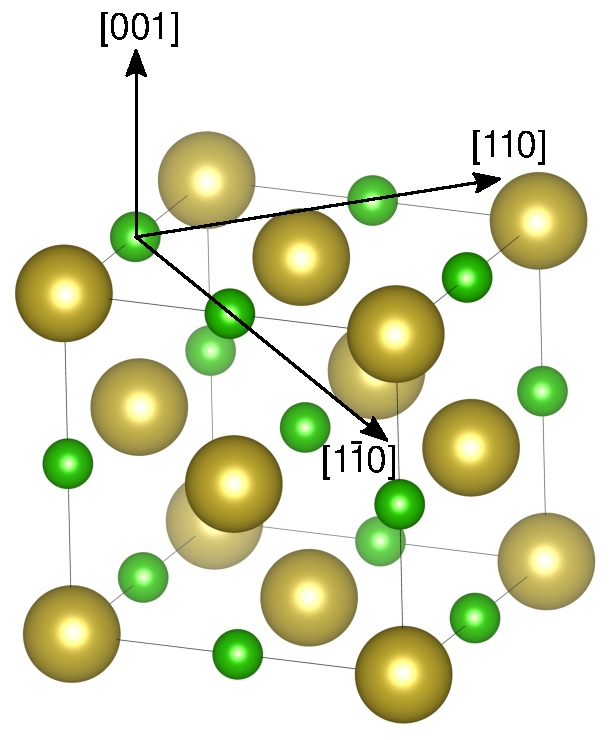
\includegraphics[width=\textwidth]{NaCl_conventional_unit_cell}
    \caption{The conventional unit cell of sodium chloride with the salient slip directions and plane normals highlighted. \label{fig:NaCl_conventional_cell_slip_system_marked}}
    \end{subfigure}

    \begin{subfigure}{0.4\textwidth}
    \centering
    \includegraphics[height=2.0in]{NaCl_110_110}
    \caption{The sodium chloride unit cell best aligned with the <1\,1\,0>\{1\,\={1}\,0\} slip system. The new [100]' and [010]' axes are parallel to the to the \{1\,1\,0\} and \{$\bar{1}\,1\,0$\} axes of the conventional unit cell respectively.  \label{fig:NaCl_110_110_unit_cell}}
    \end{subfigure}
    ~
    \begin{subfigure}{0.4\textwidth}
    \centering
    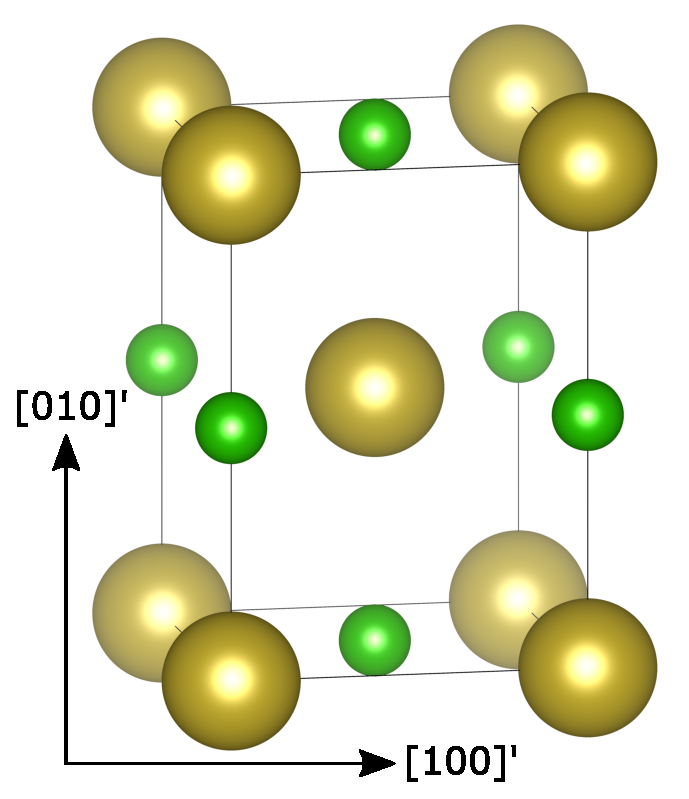
\includegraphics[height=2.5in]{NaCl_110_001}
    \caption{The sodium chloride unit cell best aligned with the <1\,1\,0>\{0\,0\,1\} slip system.  The new [100]' and [010]' axes are parallel to the to the \{1\,1\,0\} and \{0\,0\,1\} axes of the conventional unit cell respectively.\label{fig:NaCl_110_001_unit_cell}}
    \end{subfigure}

\caption[Unconventional unit cells of rock salt to build a dislocation.]{Possible unit cells for sodium chloride showing the conventional unit cell and two unconventional unit cells with the new crystallographic axes aligned to slip system, i.e. the Burgers vector and slip plane normal. Graphics prepared with VESTA \cite{Momma2011}.\label{fig:unconventional_NaCl_unit_cells}}
\end{figure}






Similarly the \ce{NaCl} <1\,\={1}\,0>\{0\,0\,1\} slip system is defined by the unit cell:
\begin{equation*}
\begin{aligned}[c]
 {[1\,0\,0]}' &=\, ^{1}\!/_{2} [1\,1\,0] \\
 {[0\,1\,0]}' &=\,  [0\,0\,1] \\
 {[0\,0\,1]}' &=\; ^{1}\!/_{2} [1\,\overline{1}\,0] \\
\end{aligned}
\qquad
\begin{aligned}[c]
&\parallel \mathbf{b} \\
&\parallel \mathbf{d} \\
&\parallel \mathbf{l}
\end{aligned}
\end{equation*}
and the atoms are:
$$
motif = \begin{pmatrix}
0 & 0 & 0 & +1 \\
^{1}\!/_{2} & ^{1}\!/_{2} & ^{1}\!/_{2} & +1 \\
^{1}\!/_{2} & 0 & ^{1}\!/_{2} & -1 \\
0 & ^{1}\!/_{2} & 0 & -1
\end{pmatrix}
$$


These unit cells are shown in relation to the conventional cell in \autoref{fig:unconventional_NaCl_unit_cells}. With these unit cells we can convolve the motif with a lattice to generate an initially perfect crystal defined with respect to Cartesian axes aligned with the slip system. Two offsets are then applied; firstly the half crystal below the slip plane, which is defined by $y < 0$, will be offset in the positive $x$ direction by $b/2$ and then the entire crystal is offset to put the dislocation core in the desired location. 

The $x$ position is defined by an offset along the slip direction
of $\alpha b$, where $\alpha$ is a variable. The position of the core normal to the slip planes might be expected to be fixed by symmetry, in the case of \ce{NaCl} the core must be at a height of $d/4$ in order to be halfway between the two (0\,2\,0) layers, but it is not inconceivable that this height might vary in some crystals.

The initial positions of the atoms in the dislocated crystal are related to those of an initially perfect crystal by:
\begin{equation}
\bm{r_i^0} = \bm{r_i^{\text{perfect}}} +\begin{cases}
[-\alpha{}b, h, 0] & \quad \text{if } y_i^{\text{perfect}} > 0\\
[b(1/2 - \alpha{}), h, 0] & \quad \text{if } y_i^{\text{perfect}} < 0\\
\end{cases} 
\end{equation}

The offset to the atomic coordinates in $-\alpha{}b$ such that as $\alpha$ increases the dislocation motion is in the positive $x$ direction. The variable $h$ defines the height (i.e.\ position normal to the slip plane) of the dislocation core with respect to the unit cell. Its value may be fixed by symmetry. These offsets are shown schematically in \autoref{fig:offsets}

\begin{figure}
\centering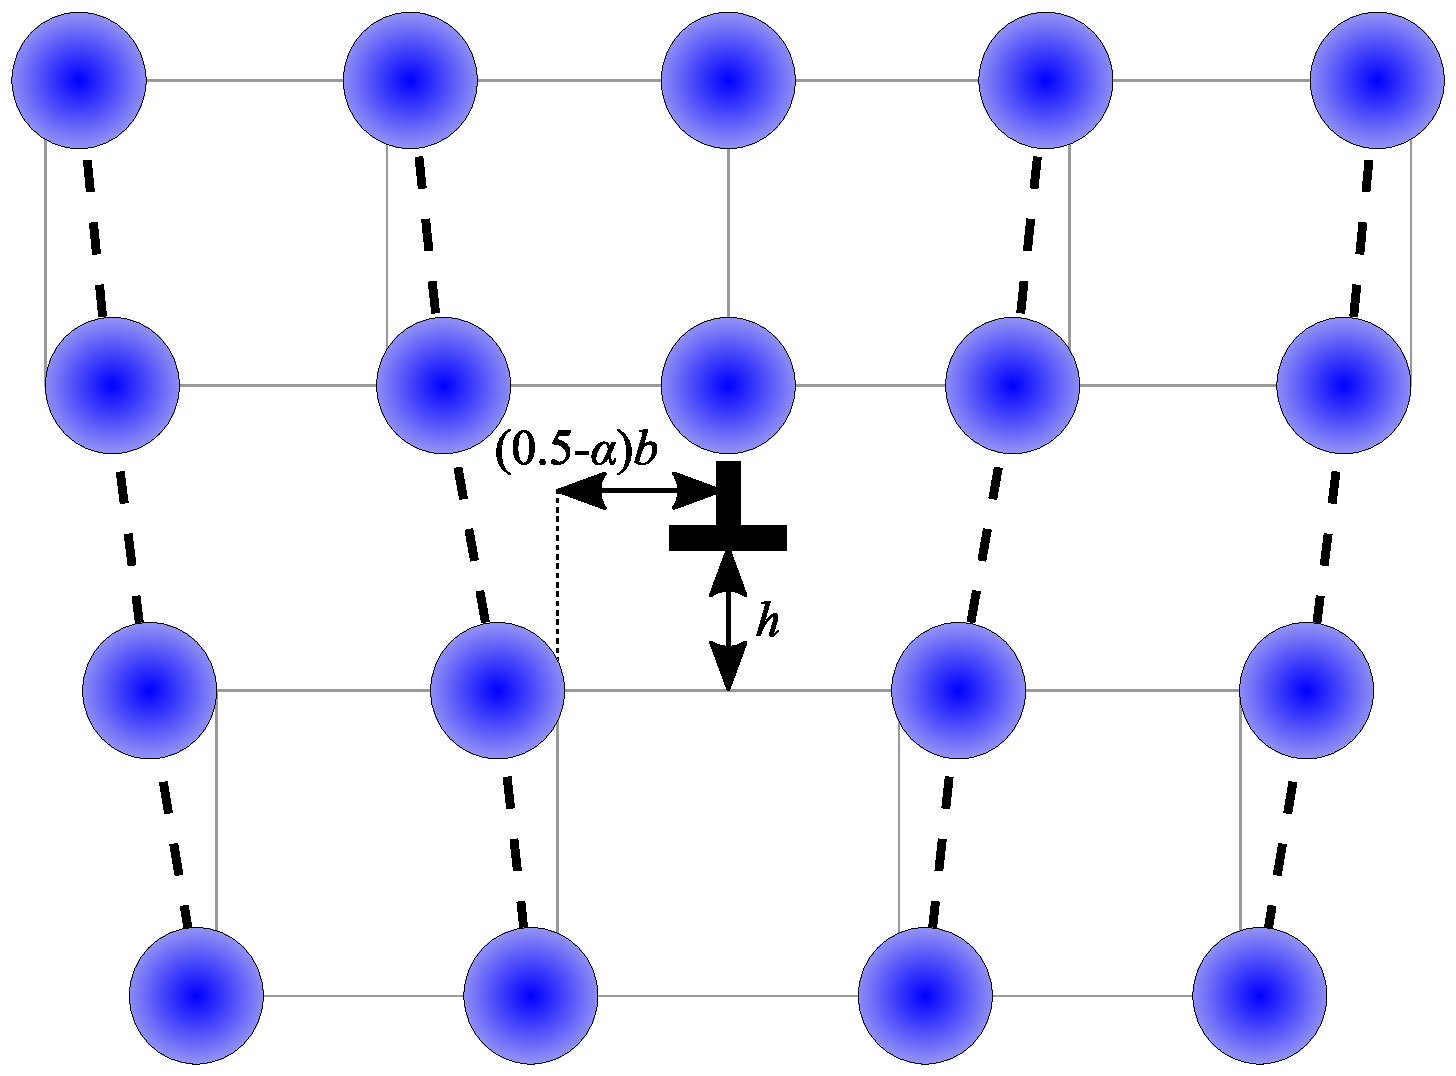
\includegraphics[width=0.7\textwidth]{Edge_Dislocation_offsets}
\caption[Schematic showing the offsets applied to position the dislocation core.]{The offsets applied to the initial atomic configuration to build a dislocation with its core centred on the correct position. The horizontal offset, i.e.\ parallel to the slip plane, is defined with respect to the lower half of the crystal. \label{fig:offsets}}
\end{figure}



\FloatBarrier












%%%%%%%%%%%%%%%%%%%%%%%%%%%%%%%%%%%%%%%%%%%%%%%%%%%%%%%%%%%%%%%%%%%%%%%%%%%%%%%%%%%

                          % Displacement fields

\subsection{Displacement fields}

A suitable displacement field is required. First we can take a Volterra dislocation, which in a continuous isotropic elastic medium has a displacement field \cite{Hirth1982Straight_dislocs}:
\begin{subequations}
\begin{align}
u &= \frac{b}{2\pi}\left[ \arctan\left(\frac{x}{y}\right) + \frac{xy}{2(1-\nu)(x^2 + y^2)} \right] \\[0.5ex]
v &= -\frac{b}{2\pi} \left[ \frac{1-2\nu}{4(1-\nu)} \ln(x^2 + y^2) + \frac{x^2 + y^2}{4(1-\nu)(x^2 + y^2)} \right]
\end{align}
\end{subequations}
where $u$ and $v$ are the components of the displacement field parallel to $x$ and $y$ respectively, $x$ is the initial position parallel to the Burgers vector, $y$ is the initial position parallel to the slip plane normal, $b$ is the magnitude of the Burgers vector and $\nu$ is the Poisson ratio of the material. The terms all converge to fixed values at large $x$ or $y$ except the logarithmic component of $v$. This represents the bending of a single crystal that arises from the introduction of an extra half plane \cite{Hirth1982Straight_dislocs}.

This formulation of the displacement field and subsequent solution for an isotropic elastic continuum is discontinuous, diverging at $r=0$, where $r=\sqrt[]{x^2+y^2}$. To remove the discontinuity \citet{Eshelby1949} proposed considering a single dislocation to be composed of a continuous distribution of dislocations with infinitesimal Burgers vectors, the integral of which yields the Burgers vector of the full dislocation. 

By considering the local strains (a normal strain parallel to the slip plane) due to this distribution, the stress on the slip plane can be found. By applying a force balance condition with the stress arising due to the misalignments, the displacements at the slip plane can be found, following the arguments laid out in \cite{Hirth_Lothe1982lattice_periodicity}. 

Let $\mathbf{b}'dx'$ be the Burgers vector of an infinitesimal dislocation lying between $x'$ and $x'+dx'$. The dislocation corresponds to a displacement of $-2(du/dx)dx'$. The total Burgers vector can be found by integration:
\begin{equation}
b = \int_{-\infty}^{\infty} b'(x') \dd x' = -2\int^{\infty}_{-\infty} \left( \! \frac{\dd u}{\dd x} \right)_{x=x'} \dd x' 
\end{equation}

The shear stress due to a Volterra dislocation  is \cite{hirth_lothe1982peierls_displacements}:
\begin{equation}
\sigma^{\text{Volterra}}_{xy} = \frac{\mu b}{2\pi (1-\nu)} \frac{x(x^2 - y^2)}{(x^2+y^2)^2}
\end{equation}
where $x$ relates to the the core of the single dislocation, centred on the origin, with Burgers vector $b$.

The shear stress on the slip plane due to a single Volterra dislocation is found, by setting $y=0$ and substituting for $b$, to be:
\begin{equation}
\sigma^{\text{Volterra}}_{xy}(x,0) = -\frac{\mu}{2\pi(1-\nu)} \int^{\infty}_{-\infty} \frac{b'}{x-x'} \!\dd x' =  \frac{\mu}{\pi(1-\nu)} \int^{\infty}_{-\infty} \frac{1}{x-x'} \left(\!\frac{\dd u}{\dd x}\right)_{x=x'} \!\dd x'
\label{eqn:elastic_stress_at_slip_plane}
\end{equation}
where $x-x'$ is the distance between some point $x$ and the infinitesimal dislocation at $x'$.

At the minimum energy position the net stress on the slip plane, i.e all $(x,0)$, vanishes, so there must be a balancing stress arising from the misalignment of the material across the slip plane. By analogy with \citet{Frenkel1926}:
\begin{equation}
\sigma_{xy}^{\text{misalignment}}(x,0) = C \sin \left( \frac{2\pi \phi}{b} \right)
\end{equation}
or in terms of the displacements either side of the slip plane:
\begin{equation}
\sigma_{xy}^{\text{misalignment}}(x,0) = -C \sin \left( \frac{4\pi u}{b} \right)
\end{equation}
If Hooke's law is satisfied at small strains we can write:
\begin{equation}
\sigma_{xy}^{\text{misalignment}}(x,0) = 2 \mu \varepsilon_{xy} = \frac{\mu{}\phi}{d}
\label{eqn:misalign_stress_at_slip_plane}
\end{equation}
We can combine \autoref{eqn:elastic_stress_at_slip_plane} and \autoref{eqn:misalign_stress_at_slip_plane} to give an integral equation thus:
\begin{equation}
\int^{\infty}_{-\infty} \frac{1}{x-x'} \left(\!\frac{\dd u}{\dd x}\right)_{x=x'} \dd x' = \frac{b(1-\nu)}{2d} \sin\left(\frac{4\pi{}u}{b}\right)
\end{equation}
A solution is \cite{hirth_lothe1982peierls_displacements, Eshelby1949}:
\begin{equation}
u(x) = -\frac{b}{2\pi} \arctan \left( \frac{x}{w} \right)
\label{eqn:one_dimensional_displacements}
\end{equation}
where $w$ is the half width of the dislocation and, for an isotropic elastic solid, has the value:
\begin{equation}
w = \frac{d}{2(1-\nu)}.\label{eqn:half_width}
\end{equation}
\autoref{eqn:one_dimensional_displacements} satisfies the boundary condition that $u(\infty) = - u(-\infty) = -b/4$. $x=w$ gives $u(w)=1/2\, u(\infty)$, i.e. in the region $-w < x < w$ the disregistry across the slip plane is greater than half the maximum that occurs at $x=0$.

The two dimensional case gives a displacement field \cite{Eshelby1949,Leibfried1949,nabarro1987theory}:
\begin{subequations}\label{eqn:displacements}
\begin{align}
u(x,y) &= \frac{b}{2\pi} \left( \arctan \left[ \frac{y +  w\frac{|y|}{y}}{x} \right] - \frac{\pi}{2} \frac{|y|}{y} \frac{|x|}{x} \right) + c_1 \frac{xy}{x^{2} + (y + w\frac{|y|}{y} )^2} \\
v^y(x,y) &= c_2 \frac{y(y +  w \frac{|y|}{y})}{x^2 + (y +  w \frac{|y|}{y})^2} + c_3 \ln \left| \frac{x^2 + (y +  w \frac{|y|}{y})^2}{b^2} \right|
\end{align}
\label{eqn:displacement_field}
\end{subequations}
The final atomic configuration is then defined by:
\begin{equation}
\bm{r}_i = \bm{r}_i^0 + [u_i\,\bm{\mathrm{\hat{i}}},\; v_i\,\bm{\mathrm{\hat{j}}},\; 0\,\bm{\mathrm{\hat{k}}}]
\end{equation}

These terms can be interpreted physically: the arctan term is the same as in the original Peierls treatment, representing displacements along the slip plane that alter the local misalignment across the slip plane. The terms with the prefactors $c_1$ and $c_2$ represent shear strains: the $xy$ and $yx$ shears respectively. The logarithmic term, with the prefactor $c_3$, represents the bending of the entire crystal that must arise from the introduction of an extra half plane of atoms. This logarithmic term does not converge to a constant value at large $x$ or $y$, but this is consistent with this physical interpretation as a bend in the lattice planes \cite{hirth_lothe1982peierls_displacements}.

Hence the parameters have physical interpretations: the width of the dislocation still defines the region with large disregistries, while $c_1$ and $c_2$ define the magnitude of displacements associated with shear strains around the dislocation core and $c_3$ defines the magnitude of the bending of a crystal that must arise from the introduction of an extra half plane of atoms.
To illustrate the displacements produced by these different terms some exaggerated (by a factor of ten from that predicted for an isotropic elastic medium) dislocation configurations are shown in \autoref{fig:parameters_of_the_disloc_configuration}.




\begin{figure}
\centering

    \begin{subfigure}{0.4\textwidth}
    \centering
    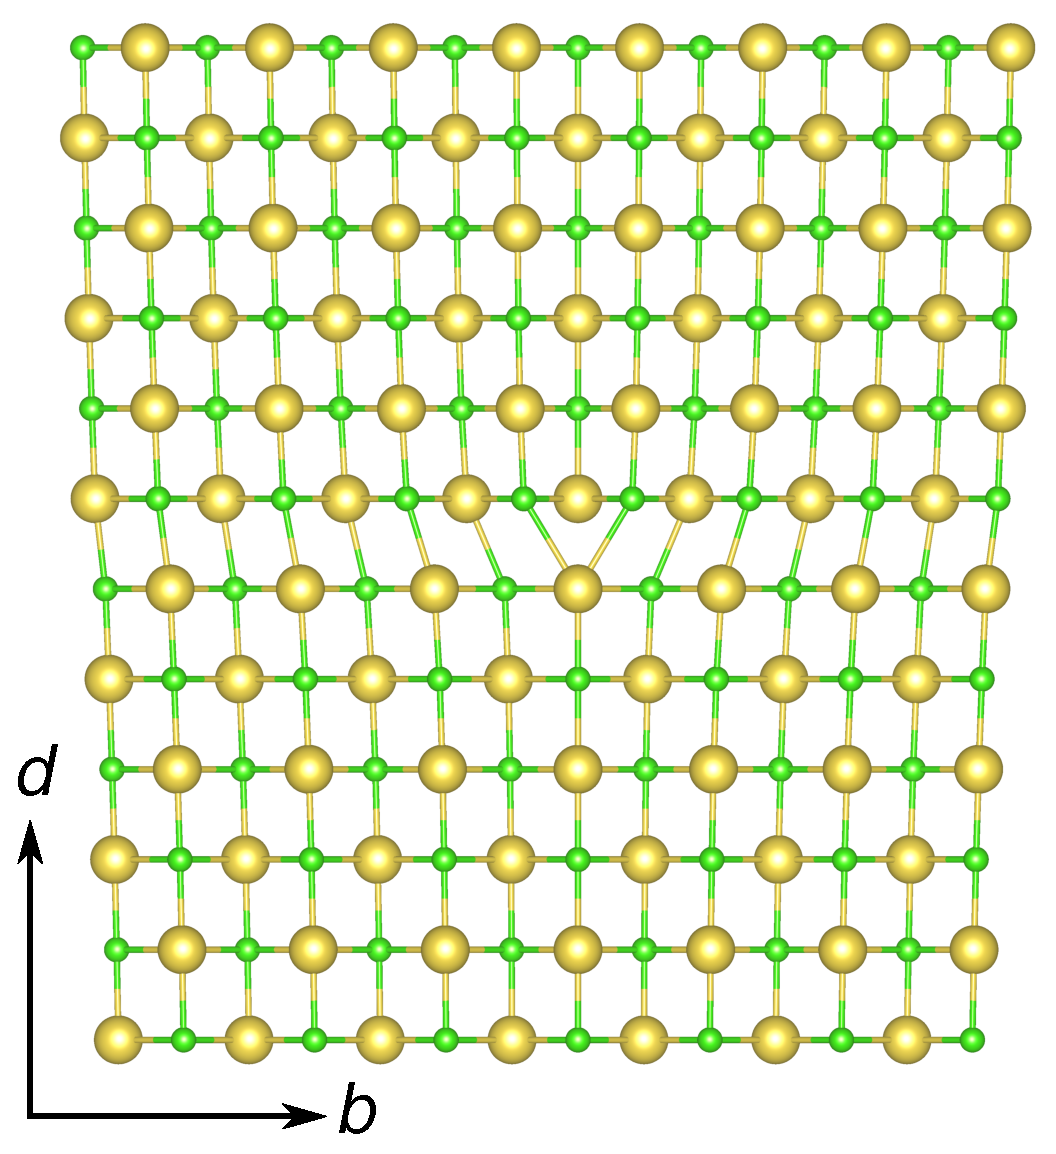
\includegraphics[width=0.6\textwidth]{wide_NaCl}
    \caption{A dislocation with a large width.}
    \end{subfigure}
    ~
    \begin{subfigure}{0.4\textwidth}
    \centering
    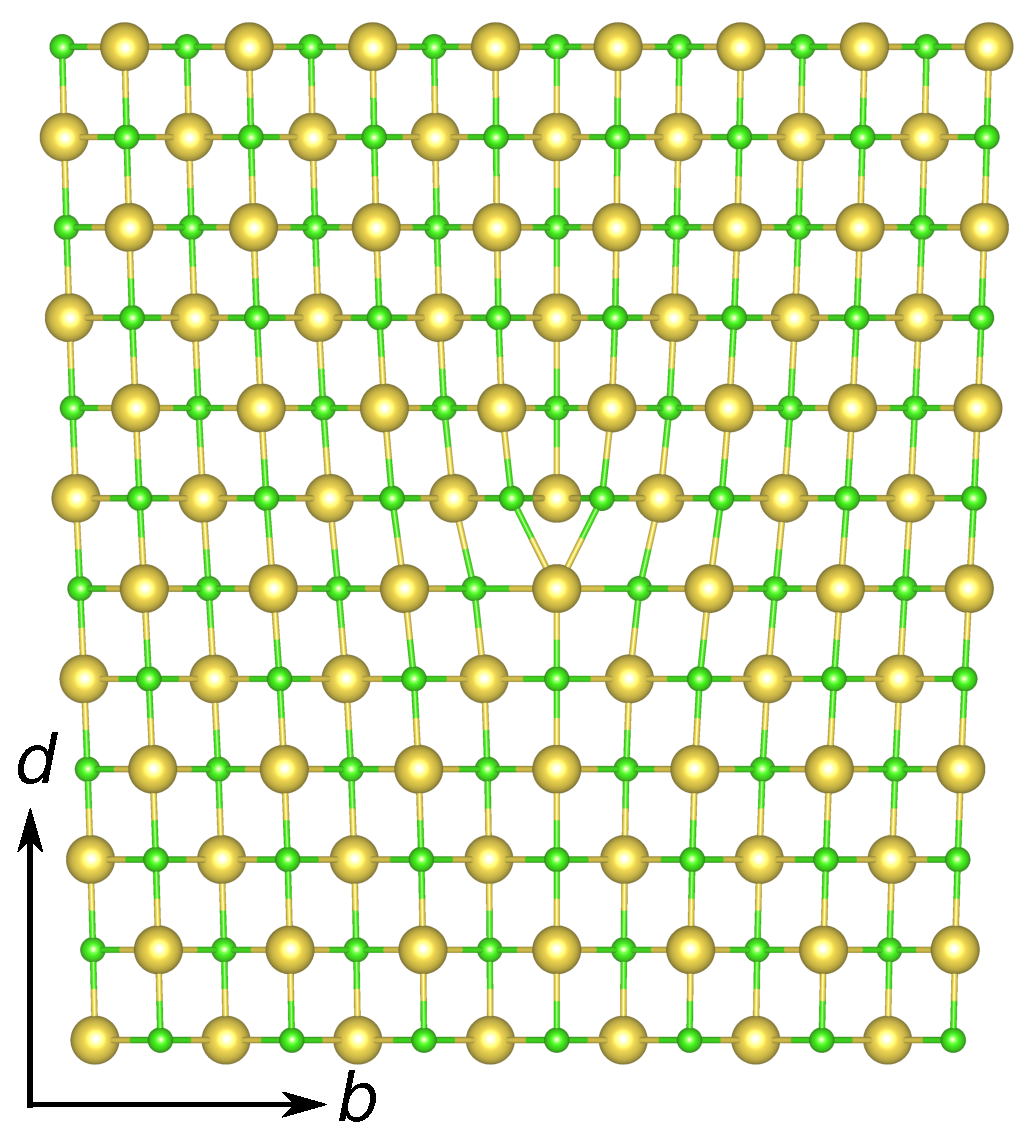
\includegraphics[width=0.6\textwidth]{narrow_NaCl}
    \caption{A dislocation with a small width.}
    \end{subfigure}

	\begin{subfigure}{0.4\textwidth}
	\centering
    \includegraphics[width=0.6\textwidth]{large_c1_NaCl}
    \caption{Large values of $c_1$ and $c_2$.}
	\end{subfigure}
    ~
	\begin{subfigure}{0.4\textwidth}
	\centering
    \includegraphics[width=0.6\textwidth]{large_c3_NaCl}
    \caption{A large value of $c_3$.}
	\end{subfigure}

    \begin{subfigure}{0.8\textwidth}
    \centering
    \includegraphics[width=0.5\textwidth]{typical_NaCl}
    \captionsetup{width=0.8\textwidth}
    \caption{A ``typical'' configuration, taken to be the dislocation structure predicted for a Volterra dislocation in a continuous elastic medium using the elastic constants of \ce{NaCl}.}
    \end{subfigure}

\captionsetup{width=0.9\textwidth}
\caption[The displacement field around an edge dislocation in rock salt.]{Various configurations of sodium chloride <1\,1\,0>\{0\,0\,1\} dislocations demonstrating the effects of the parameters of the displacement field defined in \autoref{eqn:displacements}, $w$, $c_1$, $c_2$ and $c_3$. Typical parameters are taken to be those predicted for an isotropic elastic material as given in  Equations~\ref{eqn:half_width} and \ref{eqn:disloc_params}, giving \SI{1.78}{\angstrom}, \SI{0.40}{\angstrom}, \SI{0.40}{\angstrom} and \SI{-0.12}{\angstrom} respectively for sodium chloride. Exaggerated values were ten times that. Calculated with $\nu =$~\num{0.207} and $a =$~\SI{5.644}{\angstrom} \cite{Theocaris1994,Rao1990}. Graphics prepared with VESTA \cite{Momma2011}.\label{fig:parameters_of_the_disloc_configuration}}
\end{figure}


The inclusion of $v(x,y)$ in the displacement field means that there will always be some finite displacement normal to the slip plane. This is expected and is associated with phenomena such as pressure dependent yield stress \cite{frost1982pressure}. These displacements might also be responsible for the normal strains observed around line defects in layered crystals that have been ascribed to  a new class of defect called ripplocations \cite{Gruber2016}.




For a continuous isotropic elastic medium the various parameters in \autoref{eqn:displacement_field} are found analytically  to have fixed values for the lowest energy dislocation. The half-width, $w$, takes the same value as in \autoref{eqn:half_width} and the three other parameters are defined by:
\begin{subequations}\label{eqn:disloc_params}
\begin{align}
c_1 &= \frac{b}{4\pi{}(1-\nu)} \\
c_2 &= \frac{b}{4\pi{}(1-\nu)} \\
c_3 &= - \frac{b(1-2\nu)}{8\pi(1-\nu)}.
\end{align}
\label{eqn:expressions_for_the_ideal_disloca_parameters}
\end{subequations}
The terms of the form $|x|/x$ and $|y|/y$ are to give all the terms the right sense in the right regions of space, i.e. above and below the slip plane in $y$ and either side of the dislocation in $x$. This reduces to the simpler solution in \autoref{eqn:one_dimensional_displacements} if only the atoms adjacent to the slip plane are considered. This form is useful because it is continuous and finite for all values of $x$ and $y$. 


This gives a displacement field for a general material  which has four parameters: the width, $w$, and the scaling factors, $c_1$, $c_2$ and $c_3$. These parameters are varied to find the lowest energy dislocation. If the energy is calculated by an atomistic model, rather than by continuum elasticity, then there is no analytical solution for these parameters. Instead those values that minimise the energy are taken to be the correct solution.







A final note on the parametrisation of the dislocation structure is that the values $c_1$, $c_2$ and $c_3$ are not constrained by any assumptions made so far. The purely isotropic case described above the parameters $c_1$, $c_2$ are positive and $c_3$ is negative, but there is no physical reason they cannot have a different sign. However a negative value of the width is not physically meaningful in this formulation. A negative width reintroduces the discontinuity at which displacements would diverge (in fact it would introduce two, one either side of the slip plane). Hence the constraint that $w>0$ is applied, but $c_1$, $c_2$ and $c_3$ are allowed to vary freely.





































\section{Evaluating the dislocation energy}
\label{sec:dislocation_energy}



Since there are insufficient boundary conditions to completely define a dislocation's atomic configuration with even four parameters, the energy of the dislocation is the only way to identify a correct or true configuration. Hence the energy of atomic configurations must be characterised. One method to calculate the energy is to try and replicate the model based on elastic energy in the two half crystals and misalignment energy across the slip plane. There is also the opportunity to calculate the full strain tensor and along with single crystal elastic constants the effects of elastic anisotropy can be taken into account. 

Another would be to use empirical potentials similar to those used in molecular dynamics, allowing the exploration of dislocation properties in materials that are not well modelled by elasticity or where more can be learned by other methods. Ionic solids or compound semiconductors are examples of materials where more physical insight is possible with interatomic potentials that relate more closely to the nature of the crystal chemistry than elastic constants. 



The first approach builds on the original approach of \citet{Peierls1940} and \citet{Nabarro1947} and explains how the dislocation is stable due to a balancing of two forces. There is a force that attempts to spread the dislocation out into a planar defect, which arises due to the elastic stored energy in the bonds either side of the slip plane. The elastic energy would be zero in the case of a planar defect, i.e.\ an infinitely wide dislocation. Another force tends to decrease the dislocation width, arising from the misfit or misalignment across the slip plane. The misalignment energy would be a maximum for the planar defect where the entire slip plane is misaligned and would decrease monotonically as the width decreases.

Using an elastic model to find the energy has a number of advantages. A two dimensional model is sufficient since the condition of plane strain can be applied. If elastic theory can be applied at the scale of the unit cell then displacements need only be considered between unit cells rather than within them, which simplifies the model considerably.

\subsection{Strain energy}

The elastic energy can be easily calculated for a small volume if the strain and the elastic tensor are known. A good discussion of tensors and elasticity is given by Kelly and Knowles \cite{kelly_knowles2012chapter5_tensors,kelly_knowles2012chapter6_stress_strain} and a discussion of elasticity in the context of dislocation theory is given by \citet{hirth_lothe1982elasticity}. The salient results are drawn together here.

Hooke's Law can be written as a tensor relationship using the Einstein summation convention:
\begin{equation}
\sigma_{ij} = c_{ijkl} \epsilon_{kl}
\end{equation}
where $\sigma_{ij}$ is the stress tensor, $c_{ijkl}$ is the elastic tensor defining the properties of the material and $\epsilon_{kl}$ is the strain tensor. Strain is defined, for $i=j$, by:
\begin{equation}
\epsilon_{ii} = \frac{\partial u_i}{\partial x_i}
\end{equation}
and for $i\neq j$ by:
\begin{equation}
\epsilon_{ij} = \frac{1}{2} \left( \frac{\partial u_i}{\partial x_j} + \frac{\partial u_j}{\partial x_i} \right).
\end{equation}
%In Voigt notation the equation can be written
%\begin{equation}
%\sigma_i = c_{ij} \epsilon_{j}
%\end{equation}
%where 
%\begin{equation}
%\sigma_i = \begin{bmatrix}
%\sigma_{11} \\
%\sigma_{22} \\
%\sigma_{33} \\
%\sigma_{23} \\
%\sigma_{31} \\
%\sigma_{12} 
%\end{bmatrix}
%\qquad\qquad
%\epsilon_i = \begin{bmatrix}
%\epsilon_{11} \\
%\epsilon_{22} \\
%\epsilon_{33} \\
%\gamma_{23} \\
%\gamma_{31} \\
%\gamma_{12} 
%\end{bmatrix}
%\end{equation}
%This allows the reduction of the $3\times3\times3\times3$ tensor $c_{ijkl}$ to a $6\times6$ matrix $c_{ij}$. Note that to preserve the symmetry across the leading diagonal in $c_{ij}$ the strain components for $i\neq j$ are defined by $\gamma_{ij} = 2 \epsilon_{ij}$.
If Hooke's law holds then the stored elastic energy per unit volume is:
\begin{equation}
u_{\text{elastic}} =\, ^{1}\!/_{2}\, \sigma_{ij} \epsilon_{ij} =\, ^{1}\!/_{2}\, c_{ijkl} \epsilon_{ij} \epsilon_{kl}.
\end{equation}
Hence to find the elastic energy we must evaluate \({\partial u_i}/{\partial x_j}\) for $i, j = 1, 2, 3$.
Assuming a primitive orthogonal lattice, estimating the components of strain is not difficult. The  condition of plane strain constrains $\epsilon_{ij} = 0$ for $i\, \text{or}\, j=3$. In the $1$--$2$ (or $x$--$y$) plane the strains can be identified from the vectors between neighbouring unit cells. For simplicity a primitive lattice is assumed and these vectors can be conceived of as bonds.

For this simple case two bonds are identified for each atom, one to the nearest neighbour in the $x$~direction and one to the nearest neighbour in the $y$~direction as shown in \autoref{fig:bonds}. The simplest estimate of the stress components is:
\begin{alignat}{2}\label{eqn:estimate_strains}
\left. \frac{\partial u}{\partial x}\right|_i &= \frac{\mathbf{p}_i \cdot \mathbf{\hat{i}}}{b} &\qquad\qquad
\left. \frac{\partial u}{\partial y}\right|_i &= \frac{\mathbf{q}_i \cdot \mathbf{\hat{i}}}{d} \nonumber\\
\left. \frac{\partial u}{\partial y}\right|_i &= \frac{\mathbf{q}_i \cdot \mathbf{\hat{j}}}{d} &
\left. \frac{\partial u}{\partial x}\right|_i &= \frac{\mathbf{p}_i \cdot \mathbf{\hat{j}}}{b}
\end{alignat}


\begin{figure}
\centering
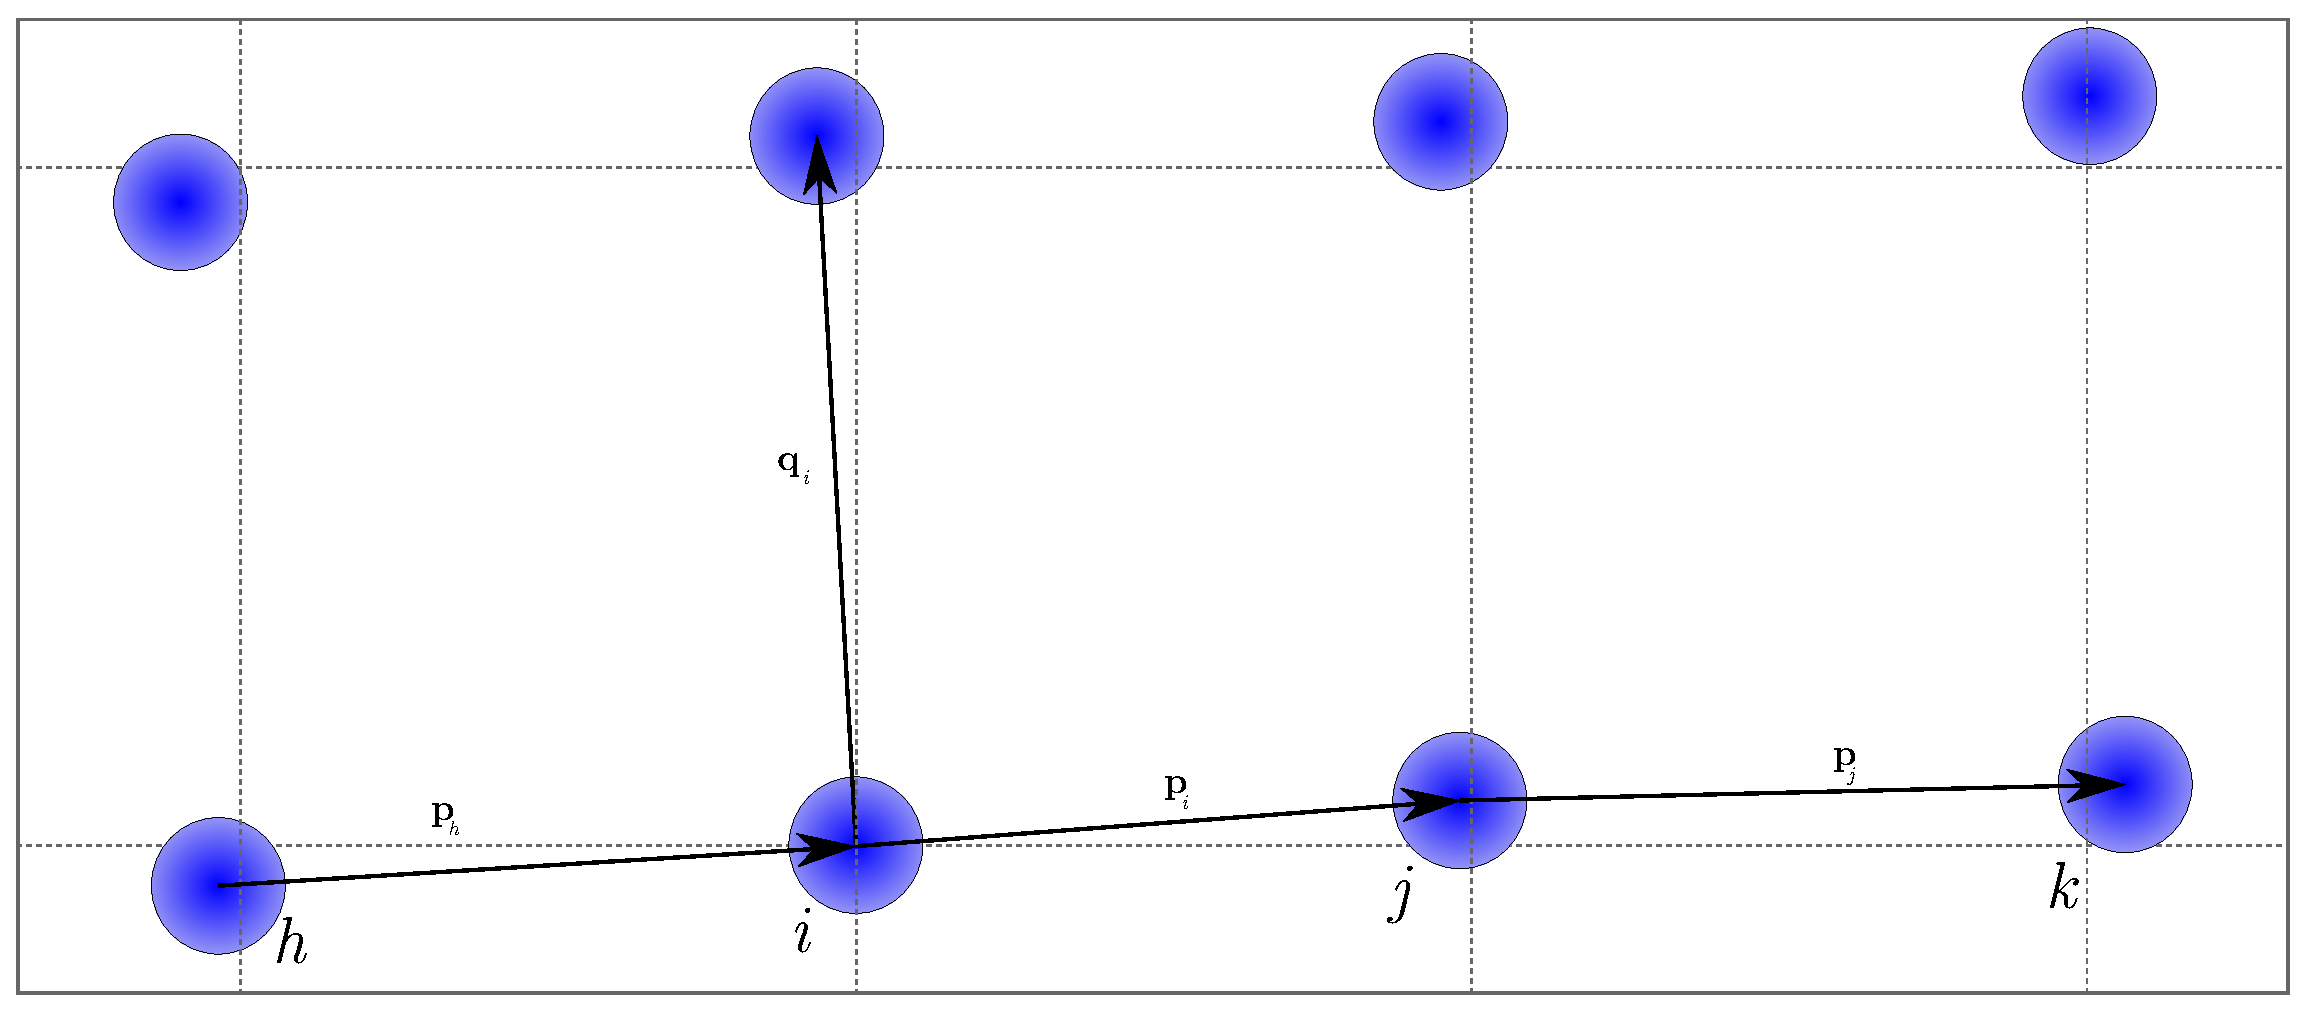
\includegraphics[width=\textwidth]{bonds}
\caption[Strained bonds in a dislocated crystal.]{The bonds that are considered for the $i$th atom in a region of crystal away from the slip plane; there is one bond to the nearest neighbour in the positive $x$~direction, $\mathbf{p}_i$, and one to the nearest neighbour in the positive $y$~direction, $\mathbf{q}_i$, to avoid double counting.\label{fig:bonds} }
\end{figure}





However there is a problem with this formulation. This assumes that every bond would, in equilibrium, be parallel to either the $x$ or the $y$ axis. This assumption is valid for the original Peierls model in which only displacements parallel to the $x$ direction were considered but the logarithmic term here represents a change in lattice orientation with position. 

Addressing this requires some estimate of the local lattice orientation. The logarithmic term in \autoref{eqn:displacements}, representing the bending of the lattice, means that far from the dislocation core the lattice can be tilted to a large angle with respect to the slip direction at the core. If the same reference axes are used everywhere, this bending results in an ever increasing strain, and therefore ever increasing strain energy away from the core. Using a local lattice orientation as the reference frame to calculate the strain means that strains will be largest near the core, as expected.


There are many possible ways of estimating the local lattice orientation. One possible method is to take the average of the neighbouring bonds so for the atom labelled $i$ shown in \autoref{fig:bonds} the ideal orientation of $\mathbf{p}_i$ would be  parallel to $(\mathbf{p}_h + \mathbf{p}_j)$. The ideal orientation for $\mathbf{q}_i$ can be taken to be at \SI{90}{\degree} to this. Therefore $\mathbf{\hat{i}}$ and $\mathbf{\hat{j}}$ in \autoref{eqn:estimate_strains} can be replaced with 
\begin{align}
\mathbf{\hat{i}}' &= \frac{(\mathbf{p}_h + \mathbf{p}_j)}{|\mathbf{p}_h + \mathbf{p}_j|} \nonumber \\
\mathbf{\hat{j}}' &= {\mathbf{\hat{i}}' \times \mathbf{\hat{k}}}
\end{align}
and the strain tensor can be calculated for each atom/unit cell, and hence the strain energy for each unit cell.




\subsection{Misalignment energy}


At the slip plane the method above will break down. For an atom immediately below the slip plane the identification of the nearest neighbour above the slip plane can be ambiguous, or can leave some atoms multiply bonded and others unbonded. The nearest neighbour will also change as the dislocation moves. \autoref{fig:slip_plane} shows an possible configuration around a dislocation core that would result in this kind of problem. Considering the atom $m$, it can be seen that it is further from both atom $i$ and atom $j$ than their other neighbours, $l$ and $n$, and so atom $m$ would be unbonded in a simple nearest neighbour model. The atom $n$ might be bonded twice in such a model.

A less arbitrary method is to use the initial positions and assume that the $i$th atom can be bonded to two atoms in the layer above the slip plane. Since initially the horizontal spacing between atoms is $b$ for all atoms the two atoms must be within an interval $x_i^0 - b < x \leq x_i^0 + b$, bonds can be identified as shown in \autoref{fig:slip_plane_initial_positions}. The energy of the two bonds is averaged to avoid a double counting error.

\begin{figure}
\centering
\begin{subfigure}{\textwidth}
\centering
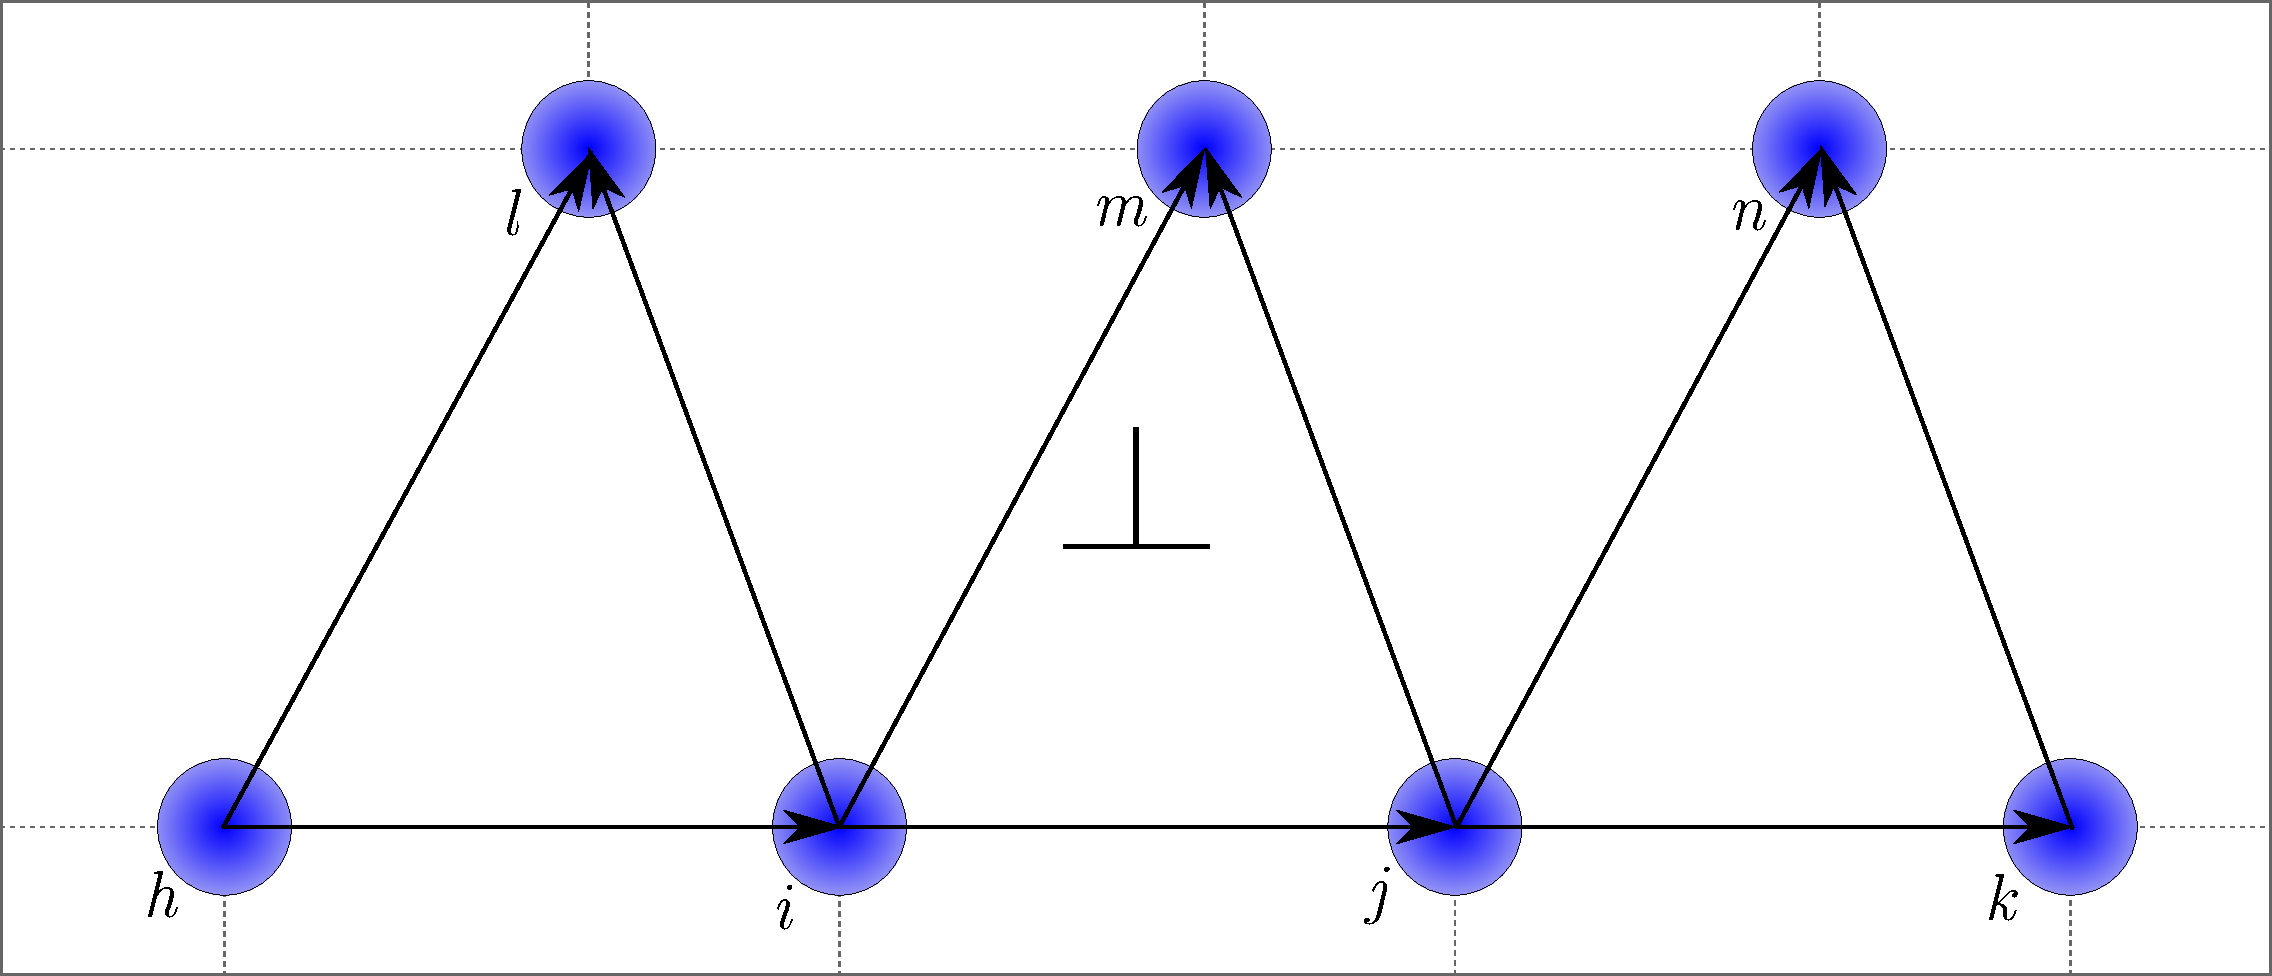
\includegraphics[width=\textwidth]{initial_slip_plane_bonds}
\caption{The initial positions of atoms either side of the slip plane.\label{fig:slip_plane_initial_positions}.}
\end{subfigure}
\par\medskip
\begin{subfigure}{\textwidth}
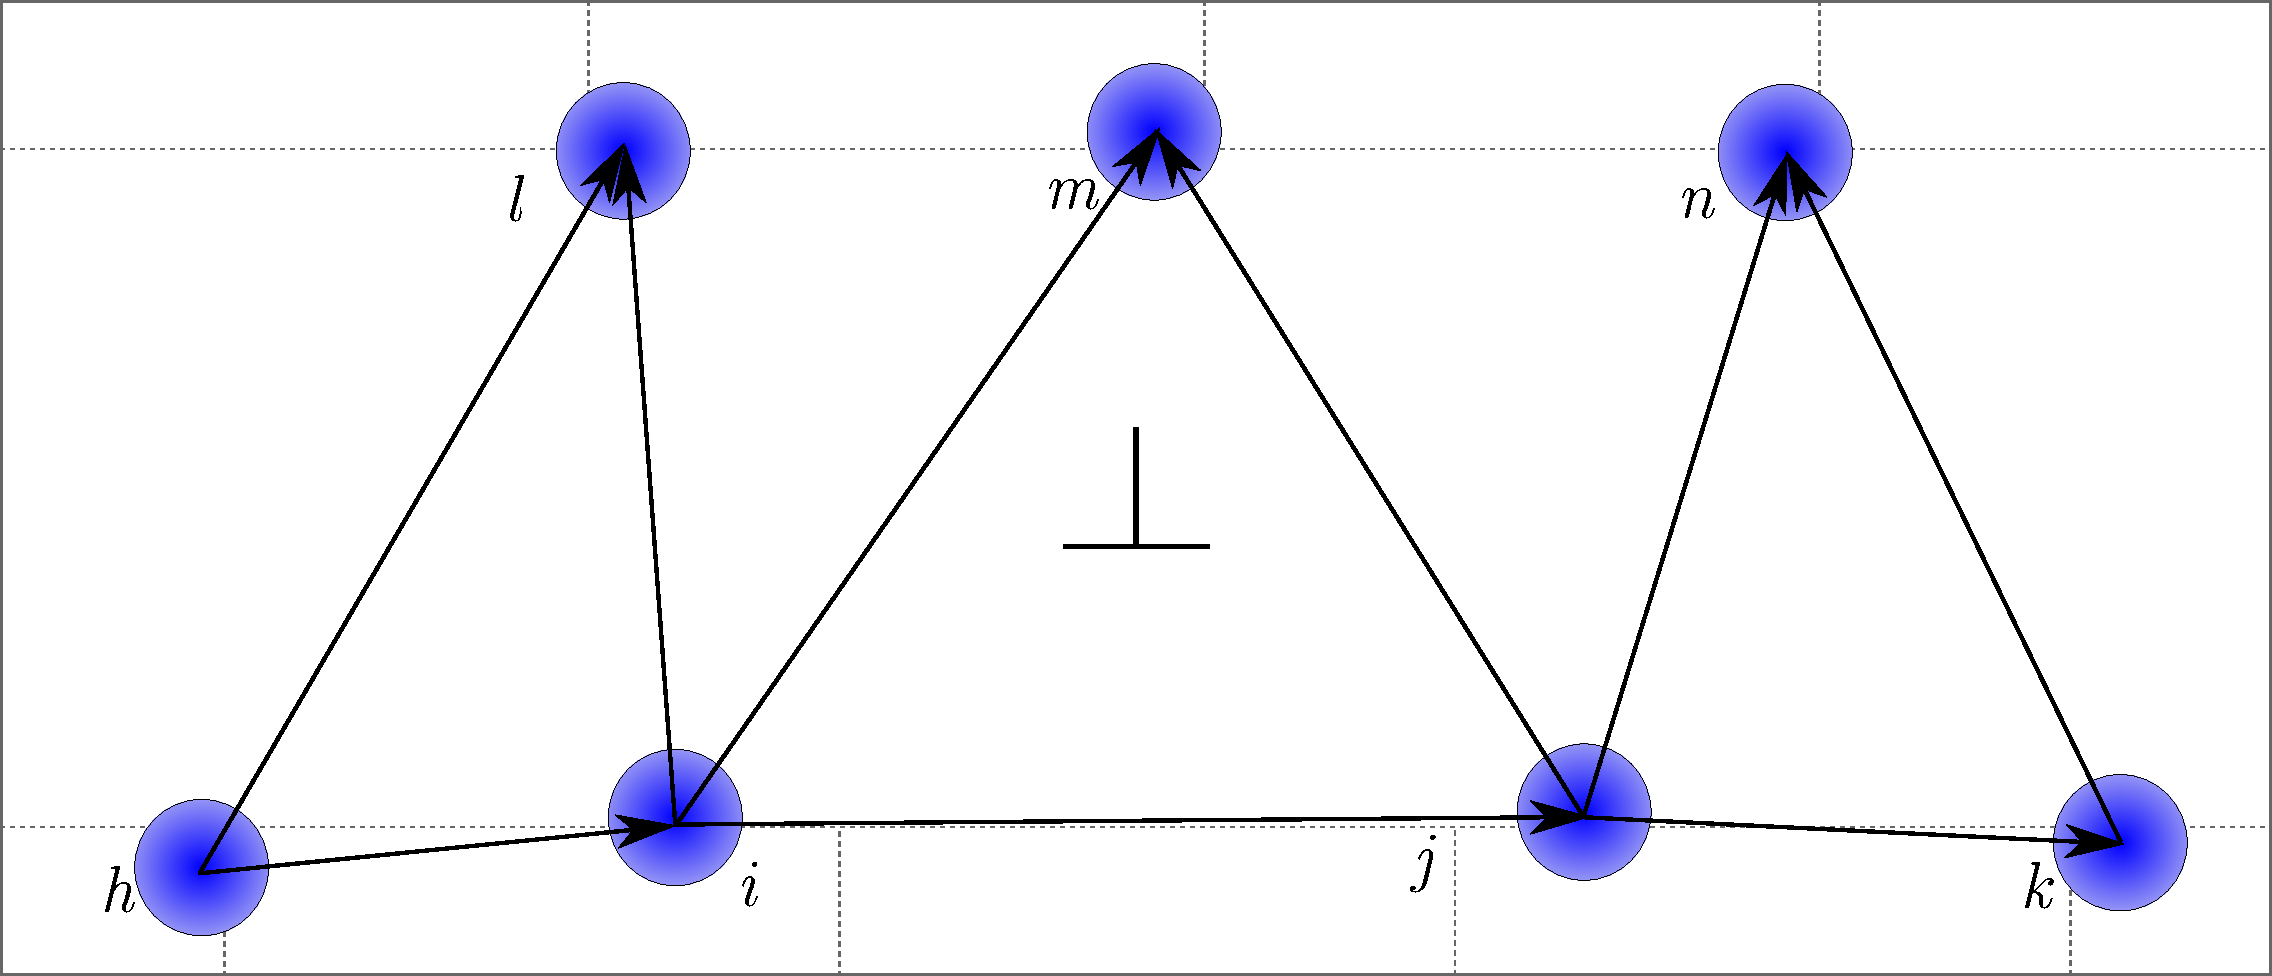
\includegraphics[width=\textwidth]{slip_plane_bonds}
\caption{The final positions of the atoms either side of the slip plane.\label{fig:slip_plane_final_positions}}
\end{subfigure}
\caption[Misaligned bonds across the slip plane.]{The slip plane before and after the application of the displacement field in the vicinity of the dislocation core. If we consider only nearest neighbours then the atom labelled $m$ would be unbonded while others, like $n$ would be bonded twice. Ambiguities can also arise when neighbours are equidistant and the neighbours would also change as the dislocation moved using a nearest neighbours model. Instead the two nearest neighbours across the slip plane are considered, as shown this results in a forward bond and a backward bond. Notice the changing orientation of the slip plane in the dislocated crystal.\label{fig:slip_plane}}
\end{figure}


There are several methods to calculate the energy of the misaligned bonds. The simplest is to use the Frenkel approximation which, for an isotropic elastic material is:
\begin{equation}
U_i^\text{mis} = \frac{Gb^2}{4\pi^2} \left[\frac{d}{b}\right] \left[ 1 - \cos \left( \frac{2 \pi \phi}{d} \right) \right]
\end{equation}
which in terms of single crystal elastic constants takes $G=C_{66}$ (in Voigt notation see \cite{kelly_knowles2012chapter6_stress_strain}). The $66$ term is used if the elastic tensor is in the frame of reference of  the slip system, with the $1$ axis parallel to the slip direction, the $2$ axis parallel to the slip plane normal and the $3$ axis parallel to the line vector. $C_{66}$ is thus always the relevant stiffness constant regardless of the material symmetry.

A more complete method for the calculation of the energy makes use of the generalised stacking fault energy. Density functional theory can be used to calculate the energy of a stacking fault at an arbitrary misalignment. This is calculated by applying a displacement to two half crystals in a DFT simulation with periodic boundary conditions which introduces two opposing planar faults. The displacement is applied along the Burgers vector and the atoms are allowed to relax perpendicular to that displacement. Although the displacement field does not include any lateral motion (i.e. parallel to the dislocation line), allowing the DFT simulation of the stacking faults to relax laterally means that the energetic implications of lateral motion are included in the misalignment potential, although with an implicit assumption that the strains along the line vector do not extend beyond the slip plane. 

The energy changes with respect to a perfect crystal were considered and fitted with a simple empirical function:
\begin{equation}
\gamma(\phi) = \sum^{M}_{m=1} C_m \left[ 1 - \cos \left( \frac{2m\pi \phi}{b} \right) \right]
\end{equation}
where $\phi$ is the misalignment in the same units as the Burgers vector $b$, $m$ is an integer from \num{1} to $M$, and $C_m$ are coefficients fitted by a least-squares method. This is in units of \si{\joule\per\square\meter}, so a factor of $b$ must be applied to convert to a line energy in \si{\joule\per\meter}.


%%%%%%%%%%%%%%%%%%%%%%%%%%%%%%%%%%%%%%%%%%%%%%%%%%%%%%%%%%%%%%%5555%%%%%%%%%%%%%%%%%%%%%%%%%%%%%%%%%%%%%%%%%






%%%%%%%%%%%%%%%%%%%%%%%%%%%%%%%%%%%%%%%%%%%%%%%%%%%%%%%%%%%%%%%%%%%%%%%%%%%%%%%%%%%%%%%%%%%%%%%%%%%




\subsection{Empirical potentials}

Some materials can be described in a more physically insightful way than linear elasticity; as described in \autoref{sec:empirical_potentials}, empirical potentials have been developed for the field of molecular dynamics to be computationally convenient while at the same time approximating reality to a sufficient degree to gain insight into a system \cite{martinez2013}. Such potentials are usually fitted to measured properties such as lattice energies and elastic constants.

One way to incorporate such potentials into the Peierls model described here is to write a simple Python implementation of the potentials using the SciPy and NumPy packages and associated tools \cite{Numpy2011,IPython2007,Millman2007,SciPy2001}; another way is to use the Atomic Simulation Environment \cite{ASE2017} or the Python interface to the LAMMPS software package \cite{Plimpton1995,LAMMPS_web}.



The ionic solids were investigated using the Lennard-Jones potential:
\begin{equation}
\phi_{ij}(r_{ij}) = 4\epsilon_{ij} \left[ \left( \frac{\sigma_{ij}}{r_{ij}}\right)^{12}-     \left( \frac{\sigma_{ij}}{r_{ij}}\right)^6   \right]
\end{equation}
where $\epsilon_{ij}$ is the depth of the energy well and $\sigma_{ij}$ is the radius at which the energy is equal to zero or in the A--B form:
\begin{equation}
\phi_{ij}(r_{ij}) = \frac{A_{ij}}{r_{ij}^{12}} - \frac{B_{ij}}{r_{ij}^{6}}
\end{equation}
where $A_{ij} = 4\epsilon_{ij}\sigma_{ij}^{12}$ and $B_{ij} = 4 \epsilon_{ij} \sigma_{ij}^{6}$. The energy for any two atoms is then: 
\begin{equation}
U_{ij}(r_{ij}) = \frac{1}{4\pi\epsilon_0} \frac{q_i q_j}{r_{ij}} + \frac{A_{ij}}{r_{ij}^{12}} - \frac{B_{ij}}{r_{ij}^{6}}
\end{equation}
where $\epsilon_0$ is the permittivity of free space.

The Lennard-Jones potential  has been chosen as a simple way to implement the application of empirical potentials. Fitted parameters are readily available \cite{Mao2014} and the potential is applicable to a class of materials for which the dislocation properties are not fully understood, the alkali halides.



\begin{table}
\centering
  \begin{tabular}{| m{3cm} | d{4} | d{-1} |}
  \hline
   Ion \rule{0pt}{3ex} & \multicolumn{1}{c|}{$\sigma_i$/\si{\angstrom}} & \multicolumn{1}{c|}{$\epsilon_i$/\si{\joule\per\mole}  }\\ \hline
   \ce{Li+} \rule{2.5ex}{0pt} & 1.715 & 241.25 \\
   \ce{Na+} & 2.497 & 327.44 \\
   \ce{K+} & 3.184 & 494.97 \\
   \ce{Rb+} & 3.302 & 1006.25 \\
   \ce{Cs+} & 3.440 & 2097.44 \\
   \ce{F-} & 3.954 & 27.05 \\
   \ce{Cl-} & 4.612 & 104.68 \\
   \ce{Br-} & 4.812 & 150.46  \\
   \ce{I-} & 5.197  & 176.56 \\
  \hline
  \end{tabular}
\caption[Lennard-Jones parameters.]{\rule[3ex]{0pt}{0pt} Parameters used for Lennard-Jones calculations from \cite{Mao2014}.\label{tab:LJ_params}}
\end{table}


The parameters used for the Lennard-Jones potential are shown in \autoref{tab:LJ_params}. These were fitted to the lattice properties of the solid salts. They are calculated for each ion individually, to best reproduce lattice properties, and must be combined according to Lorentz-Berthelot rules:
\begin{align}
\epsilon_{ij} &= \sqrt[]{\epsilon_i \epsilon_j} \nonumber\\
\sigma_{ij} &= \frac{\sigma_i + \sigma_j}{2}
\end{align}

A simple implementation without modification for computational ease, such as cut off distances, is given in \cite{code} and an example input file is given for LAMMPS in \autoref{sec:lammps_input}. LAMMPS  input files are described in the LAMMPS documentation \cite{LAMMPS_web}.

\FloatBarrier
\subsection{Optimisation of the dislocation structure}
\label{sec:optimisers}


Given one of the above cases, or a similar one, that provides energy as a function of a small number of parameters, an optimisation routine is required. The original version of this Peierls model \cite{Clegg2006} included a simple binary search to find the width of the dislocation. However for a multi-parameter space this is not appropriate.

Fortunately the open source project SciPy includes implementations of a number of optimisers. The one chosen here was the quasi-Newton method of Broyden, Fletcher, Goldfarb, and Shanno \citep{SciPy2001,nocedal2006}, or BFGS. This method uses the first derivative of the energy with respect to the different parameters, and is one of the class of algorithms known as hill-climbing optimisers, which seek a stationary point.

While the derivative of the energy with respect to the parameters is not simple to find, the atomic positions are defined as smooth functions of the input parameters and the energy is therefore likely to be a smooth function of the atomic positions too. Hence the overall behaviour of the energy as a function of the input parameters should be well suited to a gradient based method. The SciPy implementation of the BFGS algorithm includes the ability to approximate the first derivative numerically.

If it is found that the energy function is not well behaved, SciPy also includes the Nelder-Mead simplex algorithm that does not make use of gradient information. This method calculates the objective function, here the energy, at $n+1$ points in parameter space where $n$ is the number of parameters. This defines a ``simplex'', i.e. a triangle in two dimensions, a tetrahedron in three and so on. A search direction is defined along the vector joining the worst of these $n+1$ points and the centroid of the rest, and a small number of point along this line are trialled. The worst point of the initial simplex is then replaced with an ``improved'' point and the process repeated \citep{Nelder1965,Gao2012}.


\subsection{Summary}

In this section, the various constituent parts of a new Peierls model have been discussed in some detail, including how to practically implement and combine various aspects in a modular fashion. If the model is to be used in a predictive way, it should first be verified against some know benchmarks. 

Previous Peierls models have described the observed behaviour of simpler crystals well, from diamond to F.C.C. metals \cite{Bulatov1997,Clegg2006}, and so this is the natural set of benchmarks against which to test the model. Other experimental benchmarks that can be used to test the model are historical data for the alkali halides \cite{Haasen1985,Clegg2006}, which have always had problems predicting the differences between slip systems, and some more recent examples of slip in complex crystals such as cementite \cite{Stopher2017}.
























































\section{Results and Discussion}

\subsection{Elastic Energy Calculations}
\label{sec:elastic_results}
\FloatBarrier


The equilibrium dislocation configuration for a given dislocation position was calculated by optimisation of the dislocation structure with respect to the calculated energy, the sum of the strain energy in the half crystals either side of the slip plane and the misalignment energy in the slip plane. As discussed in section~\ref{sec:optimisers} the choice of optimiser is affected by the behaviour of the function. The BFGS was found to be faster than the Nelder-Mead, though both algorithms produced very similar results, within the tolerance (i.e. the error that can be tolerated) set for the algorithms to terminate. It was found that only a very small error in the result could be tolerated in deciding the algorithm had converged. Tolerating larger errors led to inconsistent results. A relative error of around \num{1e-7} was usually sufficiently low. This is important because small changes in the energy are being studied. 

The variation of the dislocation energy with respect to the dislocation parameters, as defined in \autoref{eqn:displacement_field}, was investigated. These calculations were performed for a dislocation in copper at $\alpha=0$. The simulation cell used extended to \num{800} Burgers vectors from the dislocation core, which is approximately \SI{0.4}{\micro\meter} across the whole simulation.

First the dislocation structure was optimised to find the equilibrium configuration, then the  various parameters were varied away from these equilibrium values individually. The results are shown in \autoref{fig:variation_of_U_with_params}. 


\begin{figure}
\centering
\begin{subfigure}{0.4\textwidth}
\centering
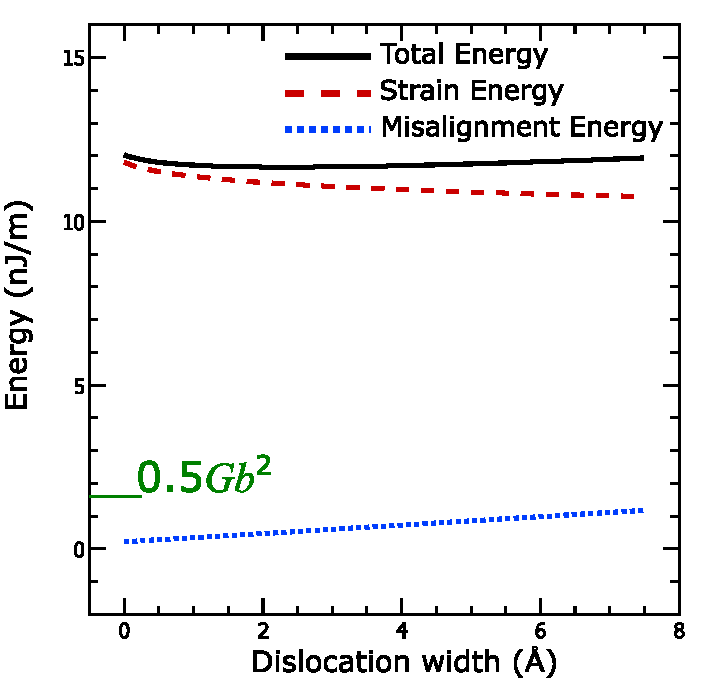
\includegraphics[width=\textwidth]{U_vs_w}
\caption{The variation in the dislocation energy with the dislocation width.\label{fig:U_vs_w}}
\end{subfigure}
~
\begin{subfigure}{0.4\textwidth}
\centering
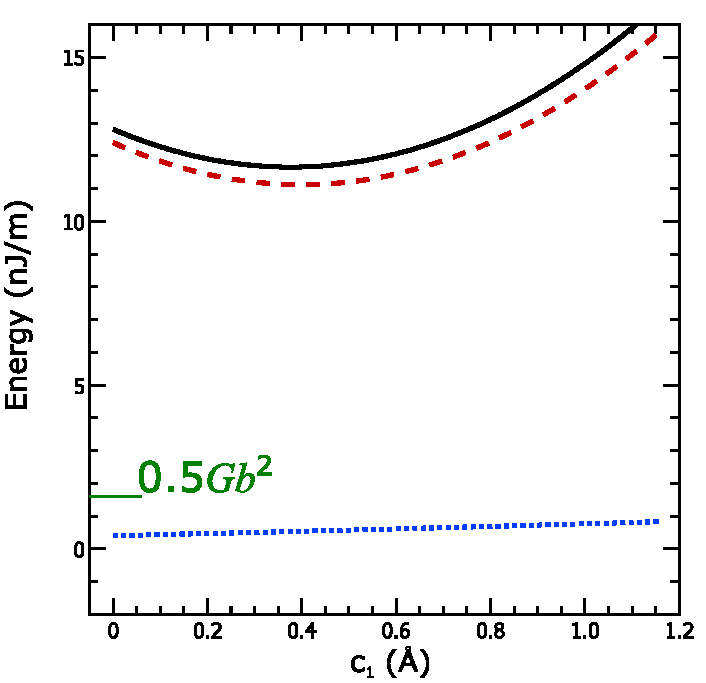
\includegraphics[width=\textwidth]{U_vs_c1}
\caption{The variation in the dislocation energy with the dislocation parameter $\mathbf{c_1}$.}
\end{subfigure}

\begin{subfigure}{0.4\textwidth}
\centering
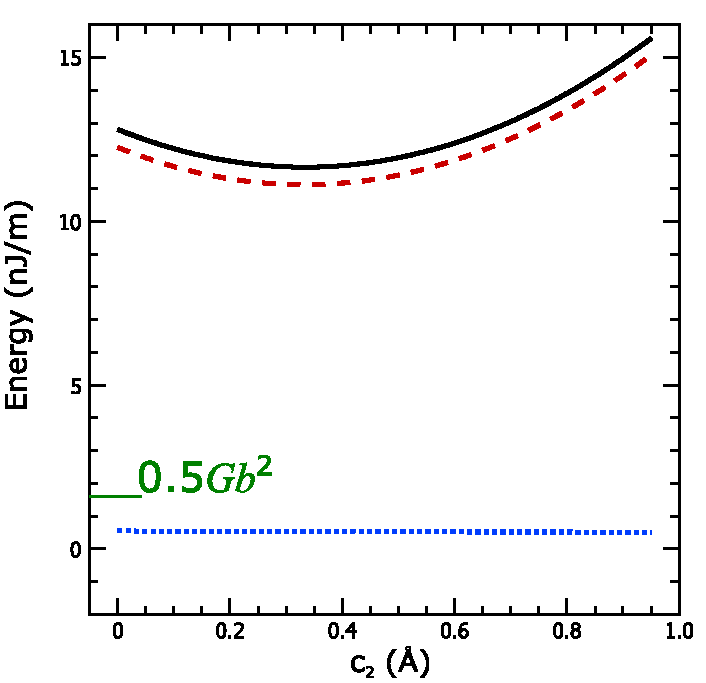
\includegraphics[width=\textwidth]{U_vs_c2}
\caption{The variation in the dislocation energy with the dislocation parameter $\mathbf{c_2}$.}
\end{subfigure}
~
\begin{subfigure}{0.4\textwidth}
\centering
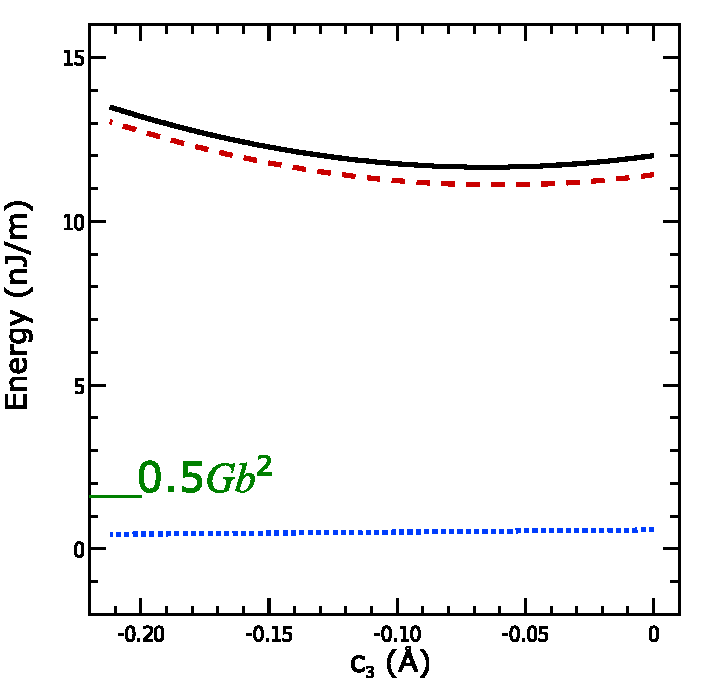
\includegraphics[width=\textwidth]{U_vs_c3}
\caption{The variation in the dislocation energy with the dislocation parameter $\mathbf{c_3}$.}
\end{subfigure}
\captionsetup{width=\textwidth,font={sf,scriptsize},labelfont=bf}
\caption[The variation of the line energy with the displacement parameters.]{The variation of the calculated energy of a dislocation in copper at the $\mathbf{\alpha=0}$ position, calculated for a simulation extending \SI{0.4}{\micro\meter} from the dislocation core. The parameters are as defined in \autoref{eqn:displacement_field}. Only one parameter was varied at a time, all the others were held constant at their equilibrium values. The total energy is the solid black line, the strain energy in the two half crystals is the dashed red line and the misalignment energy in the slip plane is the dotted blue line. \label{fig:variation_of_U_with_params}}
\end{figure}


\begin{table}[b!]


\centering
\begin{tabular}{ l c c c }
\hline
\rule[2.5ex]{0pt}{0pt}Parameter                & Ideal             & Simulated $\alpha=0$  & Simulated $\alpha=0.5$  \\
\hline
$w$ (\si{\angstrom})  \rule[2.5ex]{0pt}{0pt}   & 1.581             & 2.441                 & 2.431 \\
$c_1$ (\si{\angstrom})                         & 0.308             & 0.36268                & 0.36270 \\
$c_2$ (\si{\angstrom})                         & 0.308             & 0.293070               & 0.293075 \\
$c_3$ (\si{\angstrom}) \rule[-0.5ex]{0pt}{0pt} & -0.0493           & -0.061864               & -0.061862 \\
Energy (\si{J/m})                              &  \num{1.56795e-9} & \num{1.20965e-08}      & \num{1.20963e-08} \\
\hline
\end{tabular}
\caption[A comparison between the ideal and simulated dislocation parameters]{A comparison of the ideal dislocation parameters and those found by optimising the energy of a simulated dislocation, the ideal values of $c_1$, $c_2$, $c_3$ and $w$ are calculated from the elastic constants using \autoref{eqn:expressions_for_the_ideal_disloca_parameters}. The ideal energy is taken to be $^1\!/_2 Gb^2$.\label{tab:dislocation_params}}
\end{table}

As expected all the parameters showed a single minimum and the variation was smooth, so a variational approach is applicable and the optimiser is likely to be reliable, i.e. the lowest energy configuration can be said to be the configuration a dislocation would take. 






The values of these parameters have simple solutions for the case of an isotropic elastic medium, given in \autoref{eqn:half_width} and \autoref{eqn:expressions_for_the_ideal_disloca_parameters}. These only depend on the Poisson's ratio, which for copper is \num{\sim0.34} \cite{Koster1961}, and the lattice parameters. These ideal values are compared with the optimised values in \autoref{tab:dislocation_params}. The energy of the dislocation is approximately $4Gb^2$, higher than the $\sim0.5 G b^2$ that might be expected. However, the values of the dislocation configuration parameters are similar to the ideal values, as calculated from \autoref{eqn:expressions_for_the_ideal_disloca_parameters}. The atomistic model differs from the isotropic elastic continuum in that the values of the parameters vary as a function of $\alpha$ and the symmetry between $c_1$ and $c_2$, which are equal for an isotropic material, is broken.

The small variations in the values of the dislocation parameters and the dislocation energy, both as relative and absolute values, require that care is taken in the computation not to introduce errors. One example that has already been mentioned is the tolerance, or relative error that can be tolerated before the optimisation is terminated. If the tolerance is not tight enough,  this manifests as noise that depends on the initial guess to start the optimisation search, or the exact choices of parameters in the optimisation algorithm. This apparent noise would be deterministic but unpredictable, so would appear random. 

Another problem was the precision of the floating point arithmetic. It was found that \num{64} bit precision was usually sufficient, but some systems, particularly diamond, had such drastically different magnitudes for the strain and misalignment energies that the sum rounded to the strain energy. The dislocation energy would then be wrongly optimised to reduce that term alone. While the strain energy term dominated the line energy for these materials, principally silicon, the changes in the misalignment energy and the changes in the strain energy term were not nearly as different as the values themselves. The problem was addressed by using NumPy's \num{128} bit precision.  





\begin{figure}
\centering
% \begin{subfigure}{\textwidth}
% \centering
% 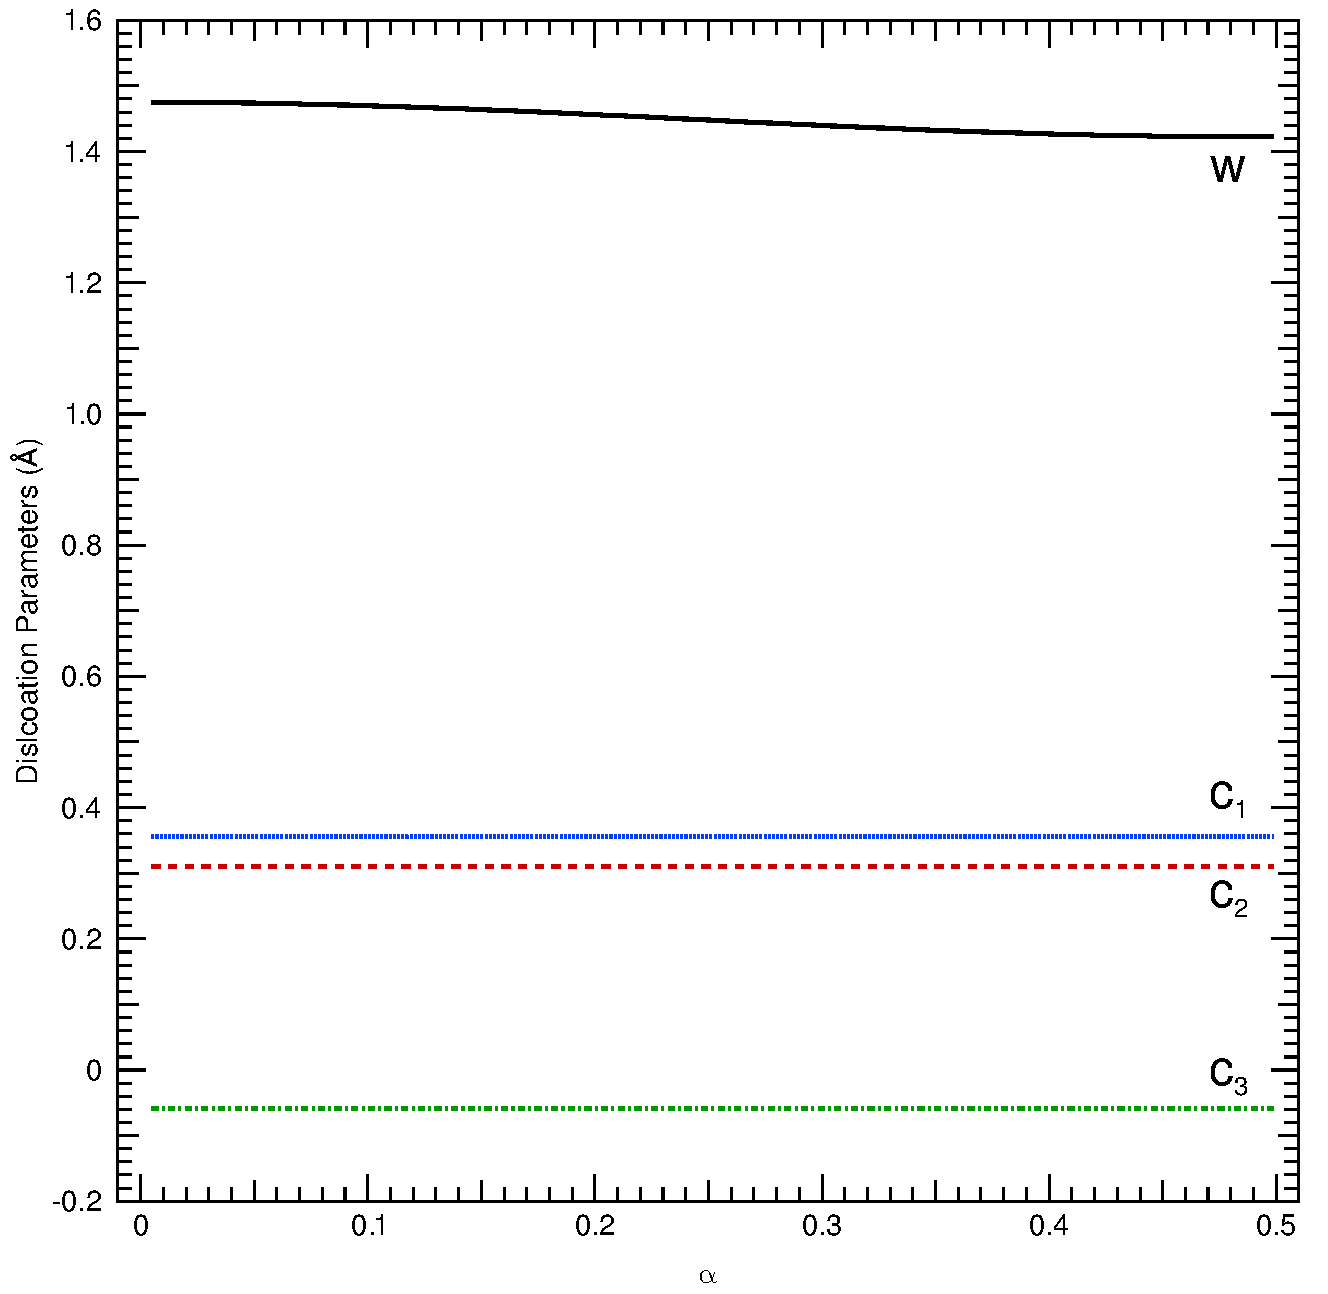
\includegraphics[width=0.6\textwidth]{disloc_params_vs_alpha}
% \caption{The variation of the dislocation configuration parameters, $\mathbf{w}$, $\mathbf{c_1}$, $\mathbf{c_2}$ and $\mathbf{c_3}$, as a function of $\mathbf{\alpha}$.}
% \end{subfigure}

\begin{subfigure}{0.45\textwidth}
\centering
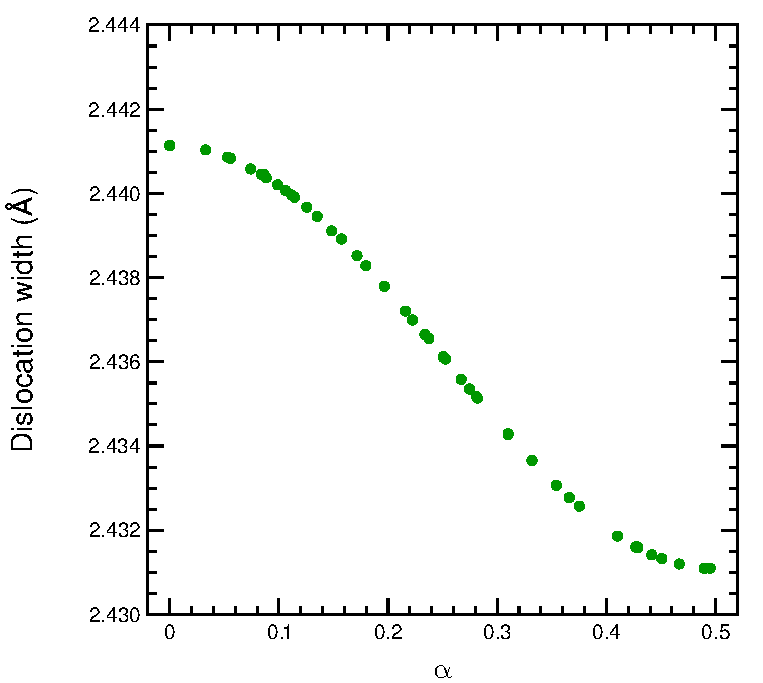
\includegraphics[width=\textwidth]{w_vs_alpha}
\caption{The variation of the dislocation width, $w$, as a function of $\alpha$. The width defines the region of the slip plane where the misalignments are greater than half the maximum value.}
\end{subfigure}
~
\begin{subfigure}{0.45\textwidth}
\centering
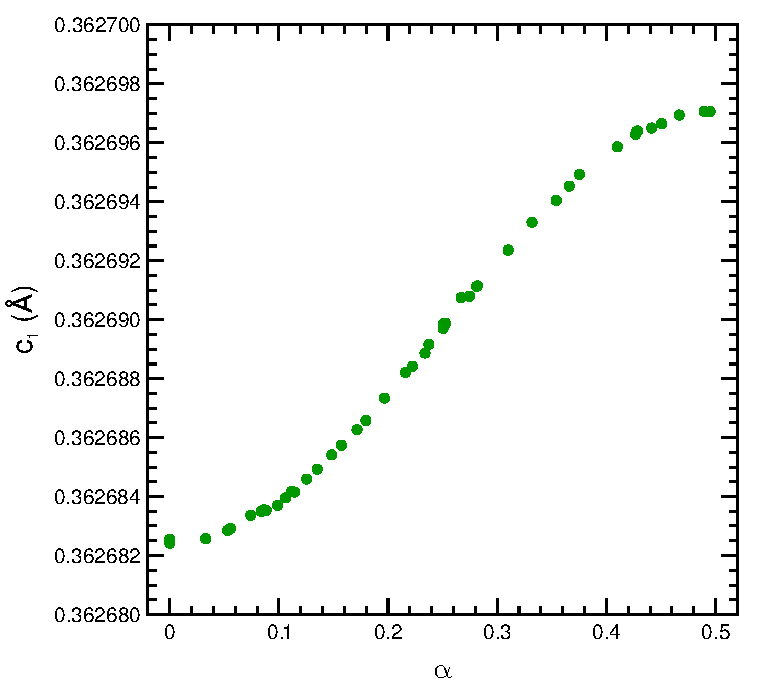
\includegraphics[width=\textwidth]{c1_vs_alpha}
\caption{The variation of the dislocation width, $c_1$, as a function of $\alpha$. The parameter $c_1$ represents the magnitude of the $xy$ strains.\rule[-\baselineskip]{0pt}{0pt}}
\end{subfigure}

\begin{subfigure}{0.45\textwidth}
\centering
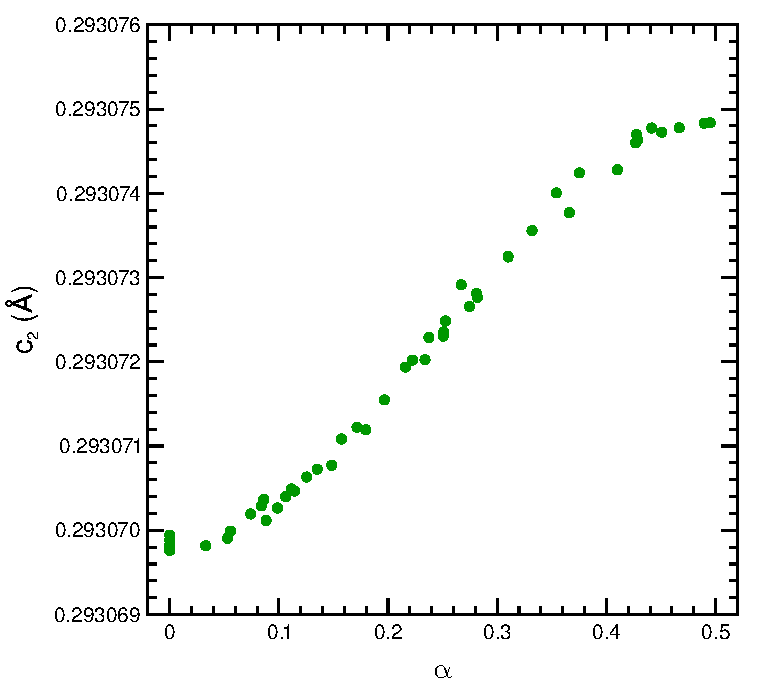
\includegraphics[width=\textwidth]{c2_vs_alpha}
\caption{The variation of the dislocation width, $c_2$, as a function of $\alpha$. The parameter $c_2$ represents the magnitude of the $yx$ strains.\rule[-\baselineskip]{0pt}{0pt}\label{fig:c2_vs_alpha}}
\end{subfigure}
~
\begin{subfigure}{0.45\textwidth}
\centering
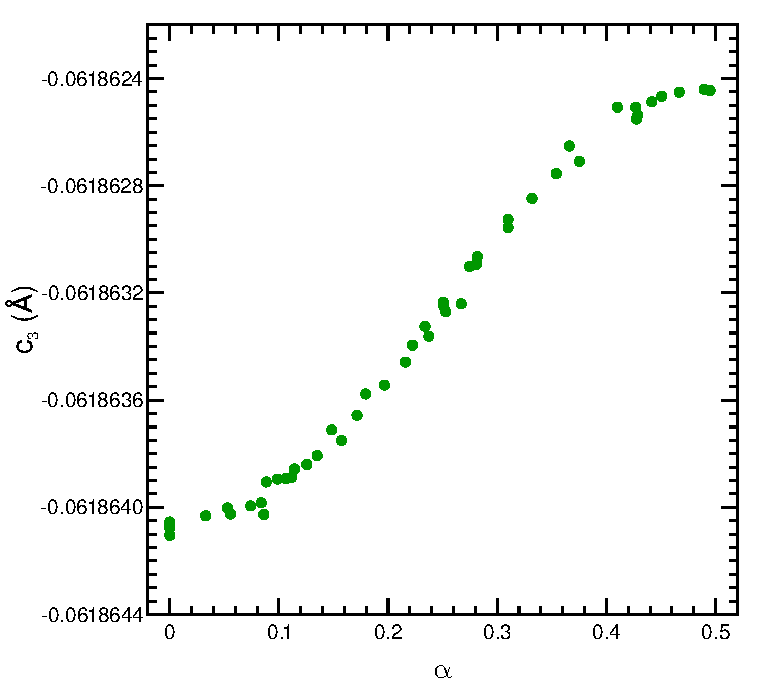
\includegraphics[width=\textwidth]{c3_vs_alpha}
\caption{The variation of the dislocation width, $c_3$, as a function of $\alpha$. The parameter $c_3$ represents the magnitude of the bending that arises in a crystal as a result of the introduction of an extra half plane of atoms.}
\end{subfigure}

\caption[The variation of the displacement parameters with dislocation position.]{The variation of the displacement field configuration parameters with $\mathbf{\alpha}$. Only small changes in the parameters were seen, the largest changes were seen in $w$ and the smallest in $\mathbf{c_3}$. The parameter all vary smoothly and approach $\mathbf{\alpha=0, 0.5}$ with no gradient, as required for equilibrium. Some noise was observed in the value of $\mathbf{c_2}$ and $\mathbf{c_3}$. \label{fig:disloc_params_vs_alpha}}
\end{figure}


The variation of the dislocation parameters and the dislocation energy were investigated by randomly sampling $\alpha$ in the range \numrange{0}{0.5} and optimising the dislocation configuration to give the lowest energy. The variation in the dislocation configuration parameters is given in \autoref{fig:disloc_params_vs_alpha}, while the variation of the total energy is given in \autoref{fig:Copper_U_tot_vs_alpha} and the relative changes in the different energy components is shown in \autoref{fig:copper_800_rel_energies}.

An important observation is that the periodicity of the dislocation energy, and indeed the dislocation configuration, predicted by this model is $b$, not $^b\!/_2$ as predicted by \citet{Peierls1940,Clegg2006}. As discussed in Chapter~\ref{chap:plastic_deformation}, this is expected based on the symmetry inherent in the model. 

Peierls introduced an implicit symmetry by assuming that the dislocation configuration does not change as the dislocation moves and thus predicted a period of $^b\!/_2$. The formulation was changed by \citet{Huntington1955} to predicted a period of $b$. The model presented by \citet{Clegg2006} included an implicit symmetry since motion of atoms was limited to the slip direction and the strain energy was calculated from strains in the atomic bonds rather than as an integral over an elastic medium. This meant that there was no distinction between the atoms above the slip plane and the atoms below the slip plane, and thus no distinction between the $\alpha = 0$ and $\alpha = 0.5$ position. The current model has no such symmetry across the slip plane, due to the logarithmic term in \autoref{eqn:displacement_field}, and so the periodicity of $b$ is expected.

The dislocation parameters vary smoothly from $\alpha = 0$ to $\alpha = 0.5$ and approach the two equilibrium positions with zero gradient as required by equilibrium. There is some noise in the value of $c_2$, as shown in \autoref{fig:c2_vs_alpha}. This is likely due to the changes in the dislocation parameters being close to the tolerance of the optimisation algorithm. This is not sufficiently noisy to present a problem, but highlights the need for care in deciding the trade off between computational time and the accuracy of the calculated values.



\begin{figure}
\captionsetup{width=0.6\textwidth,font={sf,scriptsize},labelfont=bf}
\centering
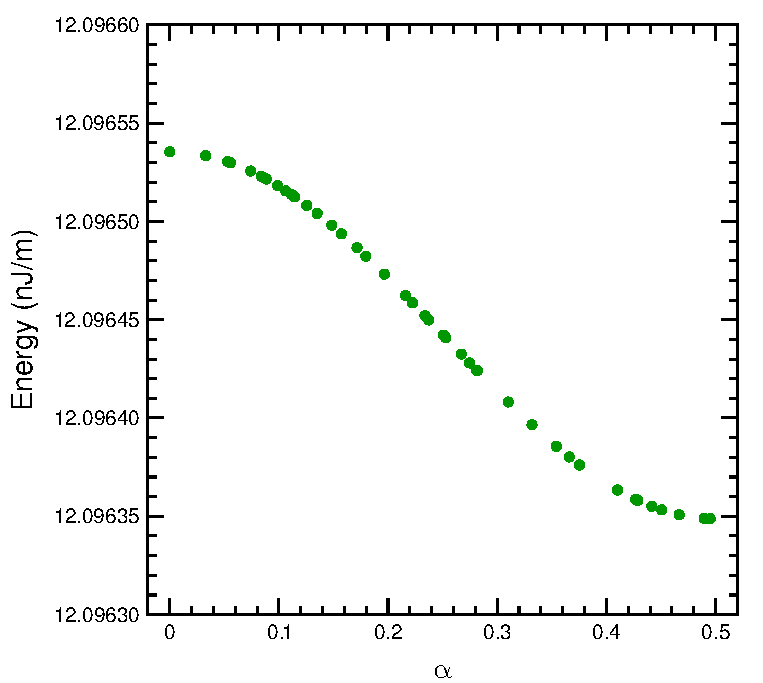
\includegraphics[width=0.5\textwidth]{Copper_800_U_tot}
\caption[Energy variation of a dislocation in copper with the dislocation position.]{The variation of the dislocation energy with position for a dislocation in copper. The results shown are for a model including atoms to a distance of 800 Burgers vectors from the dislocation core, i.e. a distance of $\sim$\SI{300}{\nano\metre}.  Note that the changes in energy are small relative to the absolute value of the dislocation energy, at around \num{1e-5}\,$U_{\text{disloc}}$.\label{fig:Copper_U_tot_vs_alpha}}
\end{figure}

The variation of the energy with $\alpha$, \autoref{fig:Copper_U_tot_vs_alpha}, was qualitatively as expected from previous work \cite{Bulatov1997,Clegg2006}: a smooth but very small variation in the energy, some five orders magnitude smaller than the value of the dislocation energy. The variation of the two components of the energy was also as expected. This is most easily seen as changes by setting the energy at $\alpha=0$ to be zero, as shown in \autoref{fig:copper_800_rel_energies}. The strain energy and the misalignment energy vary out of phase with each other, thus the two components of the energy experience larger variations than the total. It is also possible that the relative magnitude of the two components will alter which of the two equilibrium positions is stable and which is unstable.


\begin{figure}
\captionsetup{width=0.6\textwidth,font={sf,scriptsize},labelfont=bf}
\centering
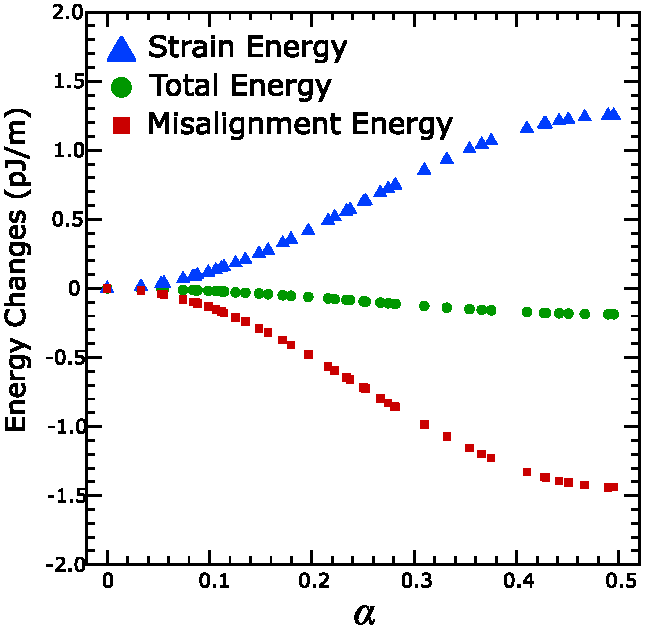
\includegraphics[width=0.5\textwidth]{Copper_800_rel_energies}
\caption[The energy changes with dislocation position for  copper.]{The energy changes with position for a dislocation in copper showing the two components of the energy, the strain energy and the misalignment energy, and the total energy. This simulation extended \num{800} Burgers vectors from the dislocation core, or around \SI{04}{\micro\meter}.\label{fig:copper_800_rel_energies}}
\end{figure}




To undertake further analysis the energy variation can be fitted with a simple empirical function:
\begin{equation}
U = \sum^N_n C_n \cos (2 \pi n \alpha) \label{eqn:empirical_function}
\end{equation}
where $C_n$ are the parameters to be fitted, $n$ is an integer between $0$ and $N$ and $\alpha$ is the displacement of the dislocation from the initial position as a fraction of the Burgers vector. Usually it was found that $N=4$ gave a good fit to the calculated energy variations. Since this is an easily differentiable function, the stress can be calculated in a straightforward manner from the gradient:
\begin{equation}
\tau = \frac{dU}{d\alpha} \frac{1}{lb^2}
\end{equation}
where $l$ is the length of dislocation line and $b$ is the Burgers vector. The gradient is readily calculated by:
\begin{equation}
\frac{dU}{d\alpha} = \sum_n^N - 2 \pi C_n \sin ( 2 \pi n \alpha )
\end{equation}

This provides a smooth and differentiable function that both allows for noise in the data and makes calculating the Peierls stress easier. The Peierls stress is the maximum value of the stress, which occurs at the point of maximum gradient $dU/d\alpha$, i.e. where:
\begin{equation}
\frac{d^2U}{d\alpha^2} = \sum_n^N -4 \pi^2 n^2 C_n \cos ( 2 \pi n \alpha ) = 0
\end{equation}

A script was written to do this fitting and gradient calculation automatically; the code is included in an archive which can be found in \cite{code}. An example of this sort of fit is shown in \autoref{fig:empirical_fit}. For the example of copper above, this yields a Peierls stress of \SI{8.98}{\mega\pascal} or, as a fraction of the shear modulus, \num{2.54e-4}\,$G$. This is approximately 10 times larger than the value estimated by experiment \cite{Wang1996}. However, for very soft materials the error in such experiments can be very large.

\begin{figure}
\centering
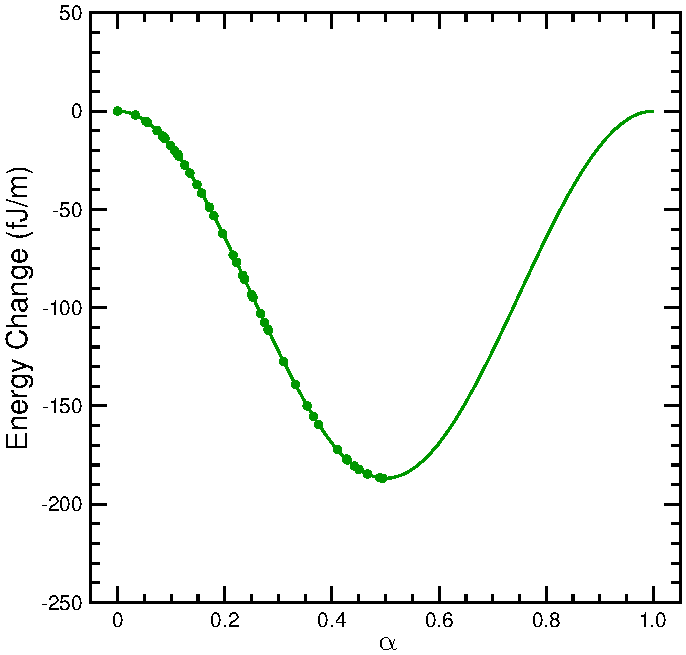
\includegraphics[width=0.5\textwidth]{Empirical_Fit}
\captionsetup{width=0.6\textwidth,font={sf,scriptsize},labelfont=bf}
\caption[Empirical fit to the variation in energy with dislocation position.]{Empirical fit to the dislocation energy as it varies with dislocation position using 4 terms. The fit is good, so can be reliably used for further analysis.\label{fig:empirical_fit}}
\end{figure}


To characterise the dependence of the model on the volume of crystal modelled, various simulation sizes were modelled for dislocations in copper. The size here is the range about the core of the dislocation in the slip direction and normal to the slip planes, while symmetry was exploited along the dislocation line to model only one repeat unit. The resulting simulated crystal therefore has a rectangular cross-section, rather than, say, cylindrical.

%Schematic?

\begin{figure}
\centering
\begin{subfigure}{0.4\textwidth}
\centering
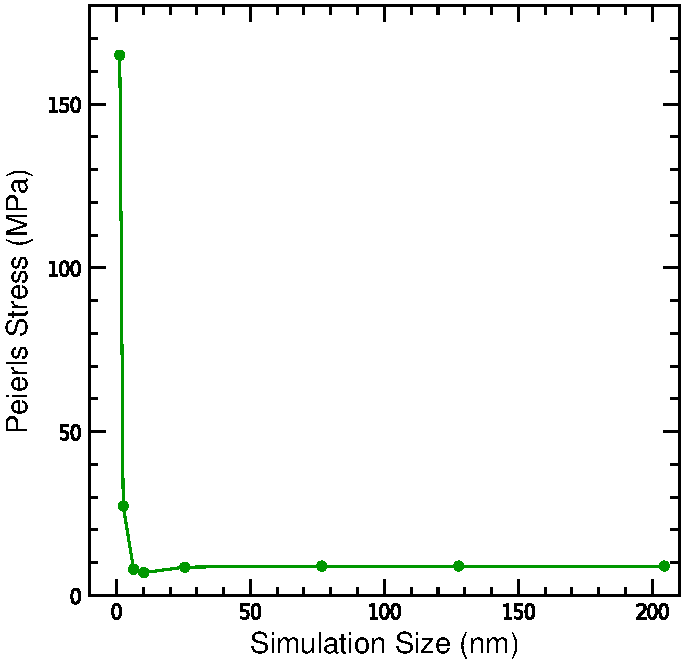
\includegraphics[width=\textwidth]{Tp_vs_size}
\caption{The variation of the calculated Peierls stress with simulation size.}
\end{subfigure}
~
\begin{subfigure}{0.4\textwidth}
\centering
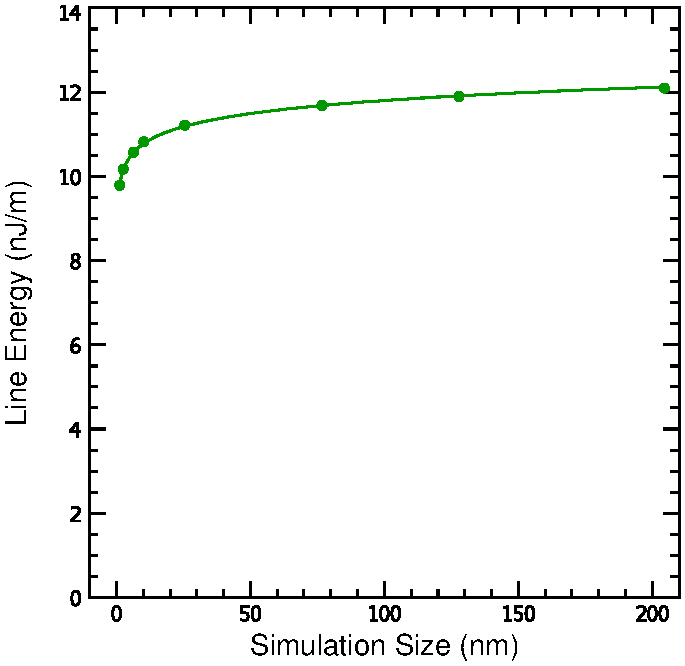
\includegraphics[width=\textwidth]{Energy_vs_size}
\caption{The variation of the calculated dislocation line energy with the simulation size and a best fit line for a logarithmic function.\label{fig:energy_vs_size}}
\end{subfigure}
\captionsetup{width=0.9\textwidth,font={sf,scriptsize},labelfont=bf}
\caption[The effect of simulation size on dislocation energy and Peierls stress.]{Plots characterising the sensitivity of the model to the simulation size. The value of the Peierls stress is quite quickly converged to a constant, the energy in fact increases logarithmically, as shown by the best fit line.\label{fig:effect_of_size_on_simulation}}
\end{figure}

\begin{figure}
\captionsetup{width=0.6\textwidth,font={sf,scriptsize},labelfont=bf}
\centering
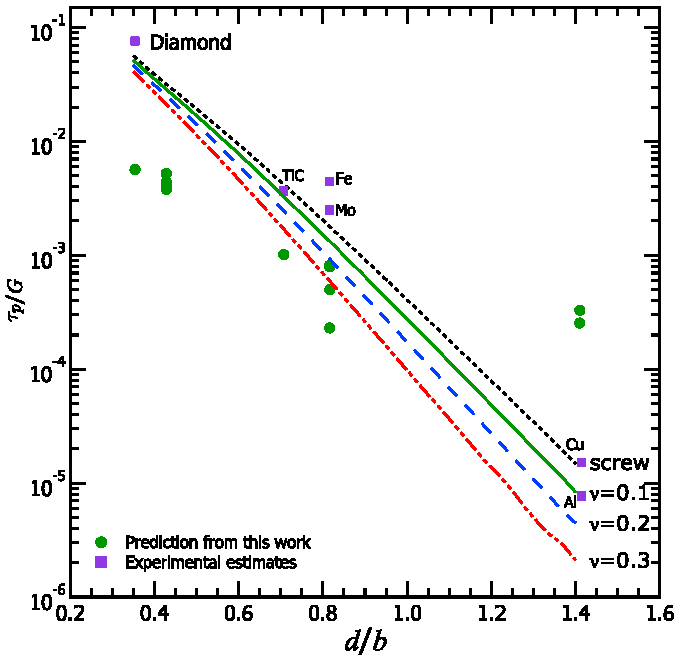
\includegraphics[width=0.5\textwidth]{tp_G_vs_d_b}
\caption[A comparison of predicted Peierls Stresses against previous estimates.]{A comparison of predicted Peierls Stresses against experimental estimates \cite{Wang1996} and a previous model \cite{Clegg2006} for an isotropic material, the highest for a screw dislocation and the others are for edge dislocations where $\nu=$ 0.1, 0.2 and 0.3. \label{fig:tp_vs_d_b}}
\end{figure}


The energy and Peierls stresses were calculated and are presented in \autoref{fig:effect_of_size_on_simulation}. The effects of size are limited to a small range for this elastic simulation, with the Peierls stress converging to \SI{1}{\percent} when the simulation is  \SI{\sim 30}{\nano\meter} across, which is around a hundred Burgers vectors.

The variation of energy with respect to simulation size does not converge, as can be seen in \autoref{fig:energy_vs_size}. However this is expected: as derived by \citet{Nabarro1947} the energy of a single dislocation in an otherwise perfect cylindrical crystal will vary logarithmically with the radius of the crystal. A best fit line is shown in \autoref{fig:energy_vs_size}, with an equation of the form:
\begin{equation}
y = c_1 + c_2 \log \left( x \right)
\end{equation}
which fits the results well. This is seen in the current work because the displacement field, \autoref{eqn:displacement_field},  includes a logarithmic term, whereas previous models have usually been limited to displacements parallel to the slip direction, at least in the far field.



The Peierls stress was calculated for a number of phases and compared with experiment and previous models, and is shown in \autoref{fig:tp_vs_d_b}. As can be seen the qualitative trends are preserved, with the same trend in Peierls stress with lattice geometry observed. However the values predicted  differ systematically from experiment: at low values of $d/b$ the current model underestimates the Peierls stress and at high values of $d/b$ the model overestimates the Peierls stress. This weaker influence of lattice geometry on the Peierls stress is consistent with previous Peierls models that have a periodicity of $b$ rather than $^b\!/_2$ \cite{Lu2000peierls}. The model is therefore limited as a quantitative predictive tool, but should allow qualitative comparisons to be undertaken.

The effect of changes in the single crystal elastic tensor were assessed for the \ce{Fe3C} structure, cementite. Work by Miles Stopher and David Bombac on the effects of hydrogen embrittlement in steels have assessed the effects of hydrogen on the elastic tensor \cite{Stopher2017}. It is expected from experiment \cite{Stopher2017} that a softening of the cementite phase occurs, allowing dislocation mediated dissolution. The elastic tensors for the four compositions, \SI{0}{at\percent}, \SI{5}{at\percent}, \SI{7}{at\percent}, \SI{10}{at\percent} hydrogen, that were investigated are given in \autoref{sec:elastic_tensors}.



The Peierls analysis results are shown in \autoref{fig:tp_cementite}. There is little to no change in the Peierls stress at hydrogen loadings of below \SI{7}{\percent}, but there is a clear and large drop in the Peierls stress for cementite between \SI{7}{\percent} and \SI{10}{\percent}. While, as seen earlier, the quantitative results of the model may not be directly comparable with experiment, the relative changes in behaviour are reliable. This is consistent with the idea that cementite is softened by the addition of hydrogen.
\begin{figure}
\captionsetup{width=0.6\textwidth}
\centering
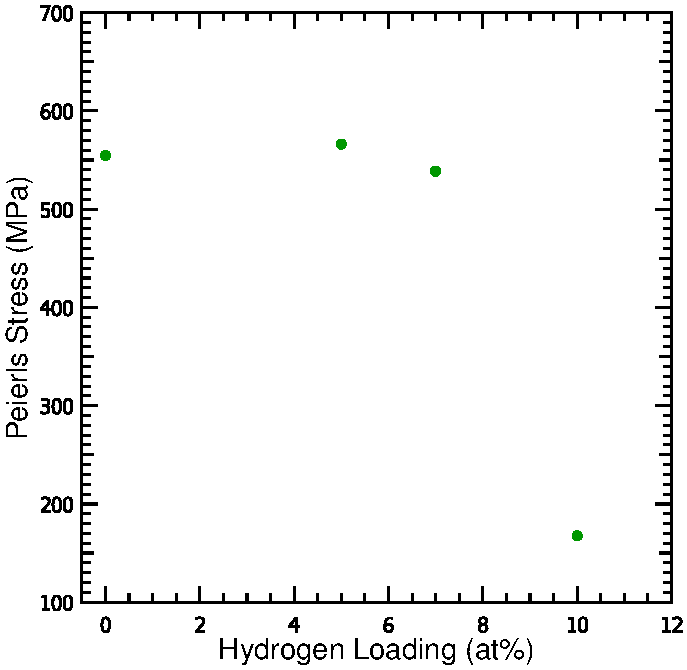
\includegraphics[width=0.5\textwidth]{Peierls_Stress_Cementite}
\caption[The effect of hydrogen on the Peierls stress of cementite]{The effect of hydrogen loading on the predicted Peierls stress of cementite on the [100](010) slip system.\label{fig:tp_cementite}}
\end{figure}


\FloatBarrier
\subsection{Dislocations in ionic solids}
\FloatBarrier


Energy changes in ionic solids were fitted with an empirical function in a similar manner to that described in section~\ref{sec:elastic_results} except now the energy components are not misalignment and strain energy terms but electrostatic and short-range terms. This was done for the two slip systems known to operate in crystals with the rocksalt structure, the <1\,1\,0>\{0\,0\,1\} and the <1\,1\,0>\{1\,\={1}\,0\}.


First the energy was calculated via a Python program, the code is available online \cite{code}, that used a simple approach: calculating the energy for all the interactions in the crystal with no cut offs. This gives the energy without the risk of artefacts that can be introduced by cut offs, but at the cost of computational time. Importantly the energy of the dislocation itself is difficult to estimate, since the energy calculated by this method includes the energy of the whole crystal, i.e.\ the energy of the free surfaces and so on. This was addressed by assuming that the energy changes were due to the dislocation alone, which is reasonable because the faces of the dislocated crystal are far enough from the dislocation not to deform very much.


The energy changes calculated in this way, using the same optimisation procedure as described above, are shown in \autoref{fig:NaCl_energy_changes}. There is a curious result that the periodicity appears to be different for the two dislocations, a period of $b$ for the <1\,1\,0>\{1\,\={1}\,0\} slip system and $^b\!/_2$ for the <1\,1\,0>\{0\,0\,1\} slip system. This can be explained in terms of the crystal structure. 

Considering the core structures shown in \autoref{fig:Schematic_NaCl_dislocs}, for the <1\,1\,0>\{0\,0\,1\} slip system the $\alpha=0.5$ position is nearly equivalent to the $\alpha=0$ position. The two positions can be related by swapping all the cations for anions and vice versa. The result is that the electrostatic energy must be the same. Since the short range potential used here is symmetrical for anion-cation or cation-anion interactions, all the first neighbour interactions will also be the same since there are no cation-cation or anion-anion neighbours to swap. There will be differences in the second nearest neighbours, which change from anion-anion to cation-cation interactions and vice versa. This difference is observed; the halfway position is lower in energy than the initial position by \SI{1.4e-22}{\joule\per\meter}. This is a very small difference as expected, but is within the expected precision of the calculation. Thus strictly the period of the dislocation energy is $b$, but for practical purposes can be treated as $^b\!/_2$. Such a similarity does not exist for the <1\,1\,0>\{1\,\={1}\,0\} slip system, so the period is more plainly $b$ without extra minima.





\begin{figure}
\centering
\begin{subfigure}{0.4\textwidth}
\centering
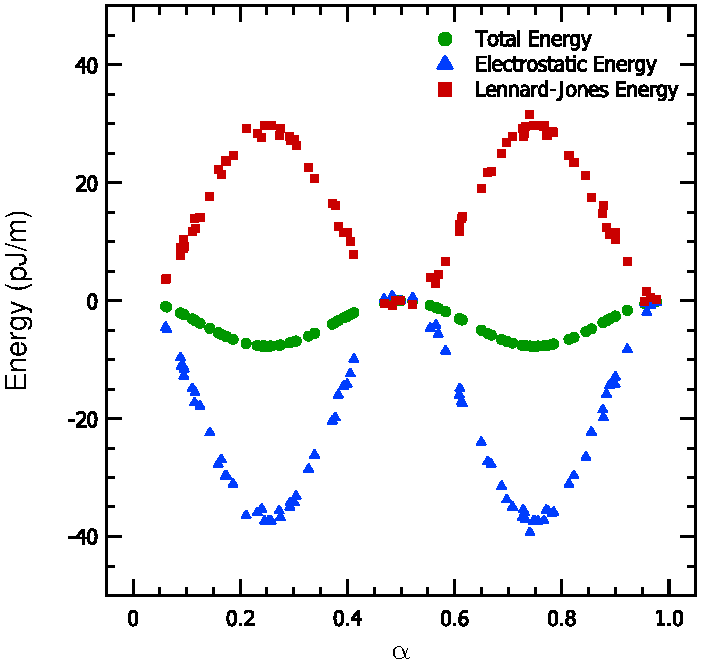
\includegraphics[width=\textwidth]{NaCl_110_001_U_vs_alpha}
\caption{The energy changes with displacement of a <110>\{001\} dislocation in NaCl.\label{fig:NaCl_110_001_energy_changes}}
\end{subfigure}
~
\begin{subfigure}{0.4\textwidth}
\centering
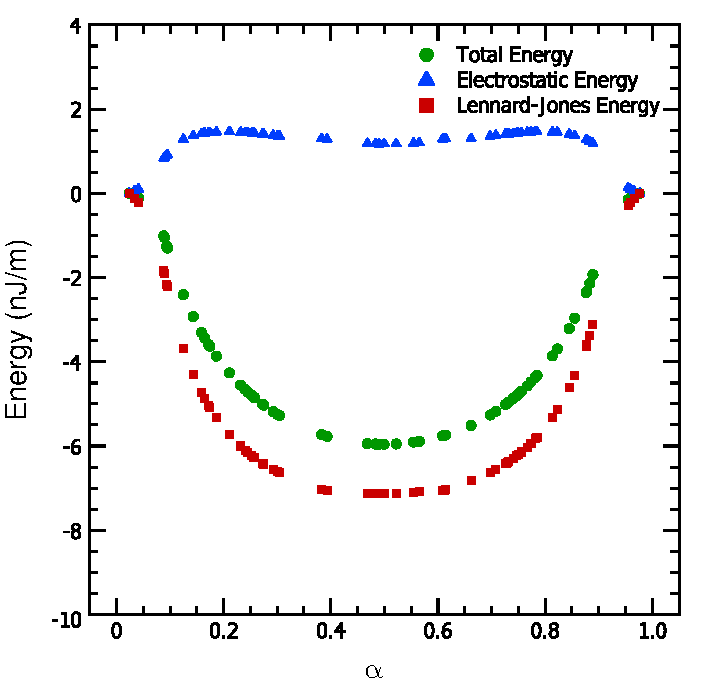
\includegraphics[width=\textwidth]{NaCl_110_110_U_vs_alpha}
\caption{The energy changes with displacement of a <110>\{1\={1}0\} dislocation in NaCl.\label{fig:NaCl_110_110_energy_changes}}
\end{subfigure}
\caption[The energy changes with position of dislocation in NaCl.]{The energy changes with position of dislocation in NaCl. Note that the scale of the energy changes is much larger for the <110>\{1\={1}0\} slip system.\label{fig:NaCl_energy_changes}}

\end{figure}



\begin{figure}
\centering
\begin{subfigure}{55mm}
\centering
\includegraphics[width=\textwidth]{zero}
\caption{}
\end{subfigure}
~
\begin{subfigure}{55mm}
\centering
\includegraphics[width=\textwidth]{half}
\caption{}
\end{subfigure}


\caption[The symmetrical positions of dislocations in NaCl.]{Dislocations in NaCl showing the similarity between the two symmetrical positions; if the short range potential were applied to only first neighbours these would be equivalent, related by reflection through the plane normal to the slip direction, in this case [1\,1\,0]. Graphics prepared with VESTA \cite{Momma2011}.\label{fig:NaCl_symmetry}}
\end{figure}


The data was fitted using the function given in \autoref{eqn:empirical_function}, and this gave the Peierls stress of the two systems as \SI{76.6}{\mega\pascal} for the <1\,1\,0>\{0\,0\,1\} slip system, and \SI{63.7}{\giga\pascal} for the <1\,1\,0>\{1\,\={1}\,0\} system. The value for <1\,1\,0>\{0\,0\,1\} system within a factor of 2 of experimental measurements of the Peierls stress, \citet{Haasen1985} estimated the Peierls stress of this slip system to be \SI{140}{\mega\pascal}. The value for the <1\,1\,0>\{1\,\={1}\,0\} slip system is clearly not in agreement with the estimated Peierls stress of \SI{10}{\mega\pascal}.



The variation of the dislocation width is shown in \autoref{fig:NaCl_w_vs_alpha}. The period of the variation of the width for the two slip systems is the same as that of the energy variation. The <1\,1\,0>\{0\,0\,1\} slip system shows the expected behaviour, small and smooth variation, as shown in \autoref{fig:NaCl_110_001_w_variation}. There is some noise in the graph showing that perhaps the model has not fully converged on the lowest energy value. There is a much larger variation in the width for the <1\,1\,0>\{1\,\={1}\,0\} slip system, \autoref{fig:NaCl_110_110_w_variation}, and there is a discontinuity in the value at around $\alpha=0.1$. This corresponds to the very steep part of the energy variation shown in \autoref{fig:NaCl_110_110_energy_changes}.


\begin{figure}
\centering
\begin{subfigure}{0.4\textwidth}
\centering
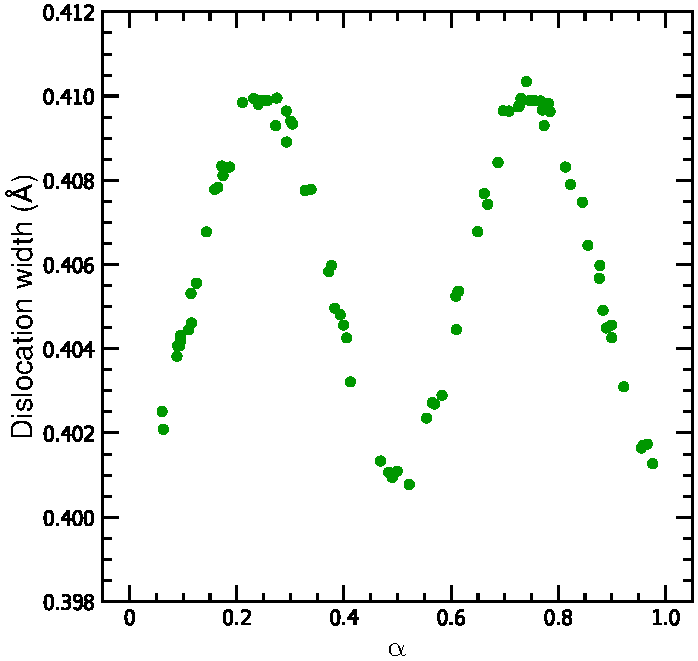
\includegraphics[width=\textwidth]{NaCl_110_001_w_vs_a}
\caption{The variation of the dislocation width with dislocation position for the <1\,1\,0>\{0\,0\,1\} slip system. \label{fig:NaCl_110_001_w_variation}}
\end{subfigure}
~
\begin{subfigure}{0.4\textwidth}
\centering
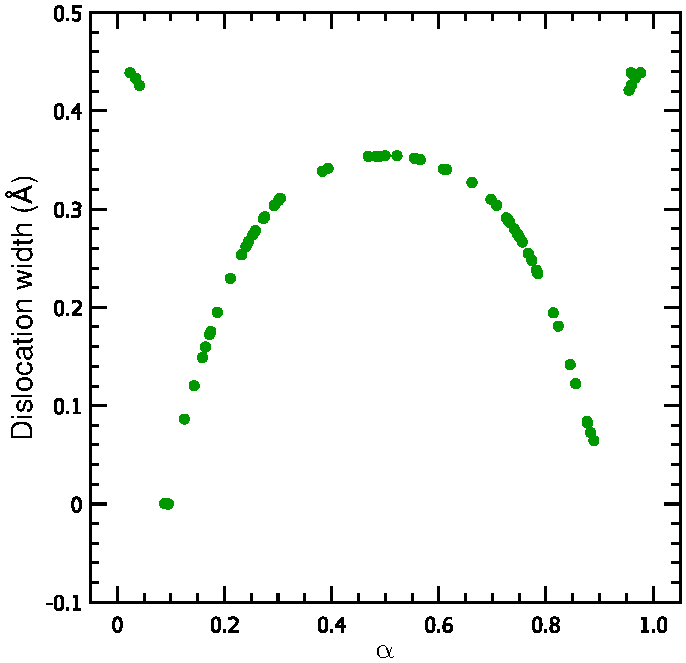
\includegraphics[width=\textwidth]{NaCl_110_110_w_vs_a}
\caption{The variation of the dislocation width with dislocation position for <1\,1\,0>\{1\,\={1}\,0\} slip system.\label{fig:NaCl_110_110_w_variation}}
\end{subfigure}
\caption[The variation of the dislocation width with position for NaCl.]{The variation of the dislocation width with position for the two slip systems of NaCl. The <1\,1\,0>\{0\,0\,1\} slip system shows the expected behaviour, showing relatively small variation in a smooth and continuous manner. The <1\,1\,0>\{1\,\={1}\,0\} slip system shows a much larger variation and a rapid if not discontinuous change at around $\alpha=0.1$.\label{fig:NaCl_w_vs_alpha}}
\end{figure}

One problem with modelling dislocations in ionic materials is the computational complexity compared to the elastic case. The model must be three dimensional since the interactions are three dimensional, which means the number of atoms is larger. Additionally the calculation scales more quickly with the size of the simulation, since now there are $n^2$ energy calculations to do for $n$ atoms rather than simply $n$ for the elastic energy calculation. Thus despite using the NumPy \citep{Numpy2011}, which is well optimised to efficiently undertake calculations, the scale of the simulation was much more limited, extending only tens of nanometers rather than hundreds from the dislocation core. Given the inherently long range nature of the electrostatic interaction this is potentially insufficient.

To address this, the model was adapted to use the LAMMPS \cite{LAMMPS_web} software package to undertake the energy calculation, using the Coulombic and Lennard-Jones calculators built in to the LAMMPS package. An example script and input files are included in \autoref{sec:lammps_input}. The principle is much the same, though now the energy calculation is using the highly optimised LAMMPS routines. These rely on choosing appropriate parameters and settings, which was done according to the LAMMPS manual \cite{LAMMPS_web}. One particular advantage is the ability to employ periodic boundary conditions along the length of the dislocation line, thus removing potential artefacts that might arise from the termination of the dislocation.

The results for the <1\,1\,0>\{1\,\={1}\,0\} slip system are shown in \autoref{fig:NaCl_110_110_U_vs_a_LAMMPS}. The variation is quite similar to that found using the na\"ive Python based energy calculator despite the periodic boundary conditions along the dislocation line and extending the simulation out from the core to \SI{\sim 100}{\nano\meter}. The maximum gradient of the best fit achievable using \autoref{eqn:empirical_function} gives the Peierls stress as \SI{63.8}{\giga\pascal}, which is very close to the the result obtained earlier, with an original calculator written in Python, as shown in \autoref{fig:NaCl_110_110_energy_changes}. 


\begin{figure}
\centering
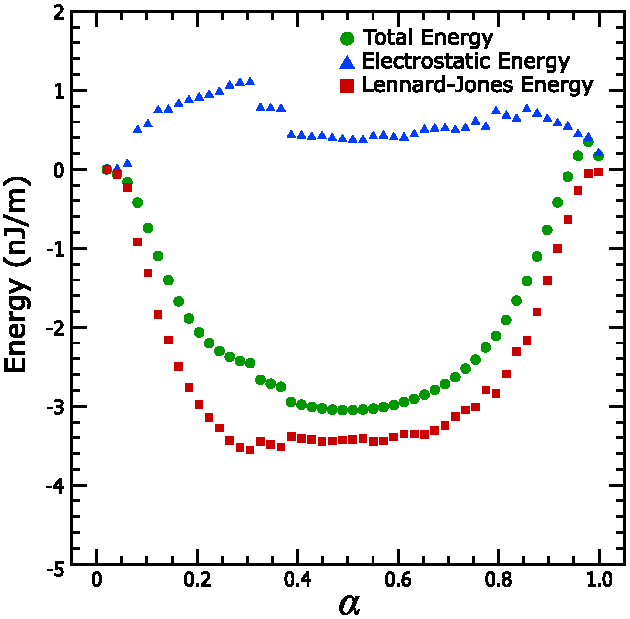
\includegraphics[width=0.5\textwidth]{NaCl_110_110_U_vs_alpha_LAMMPS}
\caption[The energy changes of a dislocation in NaCl via LAMMPS.]{The energy variation of a <1\,1\,0>\{1\,\={1}\,0\} dislocation in NaCl using the energy calculations available in LAMMPS. There is a lot of scatter, which does not appear to be random, but is likely due to insufficiently tight convergence criteria.\label{fig:NaCl_110_110_U_vs_a_LAMMPS}}
\end{figure}

The variation of the dislocation width with $\alpha$ is shown in \autoref{fig:LAMMPS_w_vs_a_NaCl}. There are some differences between the Python based model and the LAMMPS based model. Both models show a discontinuity in the width, dropping rapidly around $\alpha=0.1$, but the LAMMPS based model predicts zero width for $\alpha$ \numrange{\sim 0.1}{ 0.9}, where the Python based model predicted an increase to a maximum at $\alpha=0.5$. This might be attributable to the size of the simulation or the termination of the dislocation since those are the principle differences between the two models.

\begin{figure}
\centering
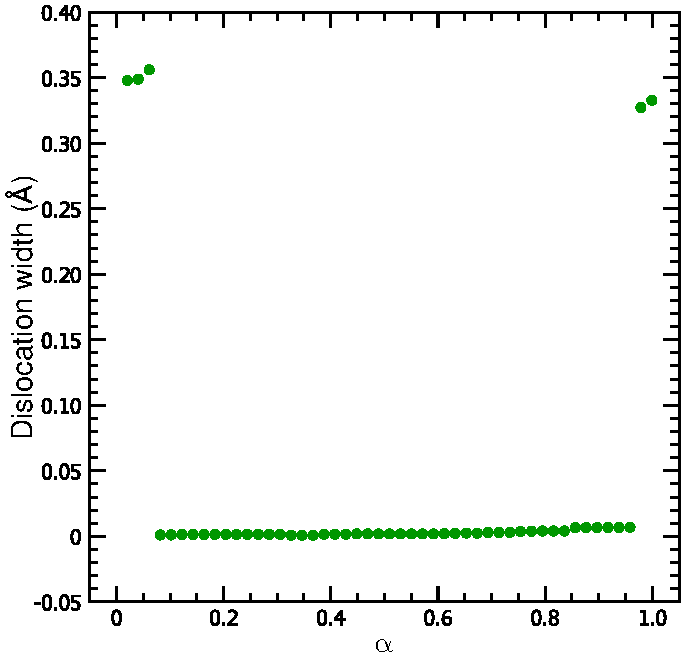
\includegraphics[width=0.5\textwidth]{NaCl_110_110_w_vs_a_LAMMPS}
\captionsetup{width=0.6\textwidth}
\caption[The variation of the dislocation width for the hard slip system in NaCl.]{The variation of the dislocation width with position for the <1\,1\,0>\{1\,\={1}\,0\} slip system in NaCl when using the energy as calculated by the LAMMPS software package.\label{fig:LAMMPS_w_vs_a_NaCl}}
\end{figure}


It therefore seems unlikely that simulation size or the termination of the dislocation at the free surface were major problems, instead some other factor is likely at fault. 

This model of a dislocation in ionic material makes a number of assumptions that it may not be valid. In the definition of the displacement field the model has assumed that all the atoms follow the same displacements that as would occur in a continuous isotropically elastic medium. This might be invalid in more than one way: firstly, there is no possibility of local deviation from the displacement field, which particularly likely to occur in the core region; secondly there is the possibility that given the long range interactions across regions of the crystals are quite unlike the elastic energy calculations used to derive the displacement field the entire form of the field may be invalid for this application. 

The second here seems unlikely given that the harder slip system was well described by the model, but the possibility of core reconstruction has been examined before, such as \citet{Hoagland1976} who observed a deviation from the ideal Volterra dislocation displacements. This could be addressed by the incorporation of more flexible boundary conditions such as those used by Hoagland \emph{et al}.

Another set of simplifications have been made in the interaction potential used here. The Lennard-Jones potential is one of the simplest potentials that can predict any material behaviour, but more accurate, if more computationally expensive, potentials do exist, incorporating the polarisability of atoms and more accurately representing the Pauli exclusion energy.

Finally there is a possible source of error in the experimental evidence for the low Peierls stress on this softer slip system. All experiments necessarily occur at finite temperatures, while the Peierls stress is by definition only valid for \SI{0}{\kelvin}. It has been observed that dislocations in alkali halides can deviate from the usual increase in critical resolved shear stress for dislocation motion as the temperature approaches absolute zero. 

There  are two effects noted by \citet{Haasen1985} that could cause the experimental estimate of the Peierls stress to be an under estimate. One effect is that the first \SI{1}{\percent} of impurity atoms can cause softening at low temperatures (<\SI{30}{\kelvin}) can make the nucleation of kinks easier and so lower the stress required to move a dislocation. The other effect  that has been suggested to explain anomalies at low temperatures is that dislocations might tunnel through the Peierls barrier in NaCL and LiF at very low temperatures (<\SI{5}{\kelvin}).




\section{Conclusions}

A parametrised form of the displacement field around an edge dislocation has been reached by adapting the solution for an isotropic elastic medium. This allows the construction of atomic configurations in three dimensions rather than one. This formulation also reduces the parameter space that must be searched for the optimal dislocation structure to a tractable size.

A series of Python modules have been written to allow the modelling of dislocations in a variety of materials using a variational approach to minimise the energy of the atomic configuration for every dislocation position. The Peierls stress is calculated from the maximum gradient of the dislocation energy. The modular nature allows functionality to be added or altered easily. 

The first module builds the dislocation by constructing an array representation of atomic coordinates around the dislocation core via the adapted displacement field. This is deliberately left extensible to allow, for example, the addition of a screw dislocation or core reconstruction.

Two further modules have been written to calculate the energy of a dislocation as represented by an array of atomic coordinates. One builds on the existing Peierls models that use linear elasticity for strain energies away from the slip plane and a misalignment potential for the slip plane, either approximated as a sinusoid that obeys Hooke's law at low strains, or fitted empirically to \emph{ab initio} calculations of the $\gamma$-surface. This module extends the Peierls analysis to use the full stiffness tensor rather than simple elastic constants. The other uses the electrostatic interaction and the Lennard-Jones potential to calculate the energy of a dislocation in an ionic solid.

The elastic Peierls model is in agreement with the trends in material behaviour observed in experiment and predicted by previous models. However the effect of lattice geometry is not as strong in this model as is observed by experiment, consistent with previous models that have a periodicity of a full, rather than a half,  Burgers vector, thus only qualitative conclusions can be drawn. The model does predict a softening of the cementite structure when hydrogen is added, as predicted by experiment.

The ionic Peierls model successfully predicts the behaviour of the <1\,1\,0>\{0\,0\,1\} slip system in \ce{NaCl} as observed by experiment. The electrostatic and short-range repulsion energy components vary out of phase with each other, in a parallel to the strain energy and misalignment energy in traditional Peierls models. The behaviour of the <1\,1\,0>\{1\,\={1}\,0\} slip system is not successfully predicted. It was shown that this was not due to the size of the simulation or the termination of the dislocation line at a free surface by the use of LAMMPS as an energy calculator, which allowed much larger simulations and the use of periodic boundary conditions. 

There are a number of assumptions inherent to the model, either implicitly or explicitly. The application of the adapted Volterra displacement field is a central assumption in this model, and this could be investigated by allowing the coordinates of atoms within some core region to relax freely while applying the displacement field to the outer regions. This is challenging due to the increased complexity of the optimisation of the dislocation structure as more parameters are allowed to vary independently. Another simplification is the use of the Lennard-Jones potential, which ignores polarisability, which is only an issue in the softer <1\,1\,0>\{1\,\={1}\,0\} slip system. More realistic potentials are available either to be implemented directly, or within projects such as LAMMPS. A final possibility that is not investigated here is the role of point defects in dislocation motion in the alkali halides. These are known to be important but the model assumes that the crystals are perfect aside from the single edge dislocation. This could be addressed with molecular dynamics, but would require significantly more computing power.






















